\documentclass{layout/tudelft-report}

%% Setting up the bibliography

% \usepackage[
% backend=biber,
% style=apa,
% citestyle=authoryear
% ]{biblatex}
% \addbibresource{report.bib}

\usepackage{biblatex}
\addbibresource{report.bib}



%% Additional packages
\usepackage{pdfpages} % Insert .pdf directly as pages
%\usepackage{minted} % Display code - use 'listings' offline without shell escape
%\usepackage[none]{hyphenat} % Disables word breaking

%% Additional commands
\renewcommand{\deg}{\si{\degree}\xspace}

%%%%% Begin of document %%%%%

\begin{document}

%% Roman numerals
\frontmatter

%% Defining the main parameters
\title{Towards Corrective Deep Imitation Learning in Data Intensive Environments}
\subtitle{Helping robots to learn faster \\ by leveraging human knowledge} % Two lines recommended
\author{Irene López Bosque}
\subject{Master Thesis}

\coverimage{figures/cover_robots_2.jpg} % Aspect ratio of 2:3 (portrait) recommended
\definecolor{title}{HTML}{d4e6ff} % Color for the title  original: 4884d6


\makecover


\begin{titlepage}

\begin{center}

%% Print the title
{\makeatletter
\largetitlestyle\fontsize{45}{45}\selectfont\@title
\makeatother}

\bigskip

%% Print the subtitle
{\makeatletter
\ifdefvoid{\@subtitle}{}{\subfont\fontsize{20}{20}\selectfont\@subtitle}
\makeatother}

\bigskip
\bigskip

by

\bigskip
\bigskip

%% Print the name of the author
{\makeatletter
\largetitlestyle\fontsize{25}{25}\selectfont\@author
\makeatother}

\bigskip
\bigskip

to obtain the degree of Master of Science \\
at the Delft University of Technology, \\
to be defended publicly on Thursday May 14, 2021 at 01:00 PM.

\vfill

%% Print some more information at the bottom
\begin{tabular}{lll}
    Student number: & 5051487 \\
        Project duration: & \multicolumn{2}{l}{January, 2021 -- November, 2021} \\
    Thesis committee: & Dr.\ ir.\ J.\ Kober, & TU Delft, supervisor \\
        & Dr.\ C.\ Celemin Paez, & TU Delft, supervisor \\
        & Ir.\ R.\ Pérez Dattari , & TU Delft, supervisor
\end{tabular}

\vspace{1cm}
\small{Cover Image: "Two robot arms" by David Levêque, found on Unsplash}

\end{center}

%% Insert the TU Delft logo at the bottom of the page
\begin{tikzpicture}[remember picture, overlay]
    \node at (current page.south)[anchor=south,inner sep=10pt]{
        
\includegraphics{layout/tudelft/logo-black}
    };
\end{tikzpicture}

\end{titlepage}

\chapter*{Abstract}
%\addcontentsline{toc}{chapter}{Abstract}


This document presents the preliminary literature review for the master thesis \textit{Towards Off-Policy Corrective Imitation Learning} whose objective is to improve the \textit{experience replay} implementation of the D-COACH (Deep COrrective Advice Communicated by Humans) algorithm; D-COACH is a framework in the field of Corrective Imitation Learning (CIL), where an agent is trained with feedback that a teacher provides in the form of relative corrections. Experience replay improves the sample efficiency by allowing already collected data to be used multiple times for training.  This is particularly important when training neural networks (NN) because it increases their stability helping to preserve old knowledge and thus reducing catastrophic forgetting. Furthermore, experience replay provides uncorrelated data to train the neural network which helps to generalize and to minimize overfitting. In order to use the experience replay technique, it is necessary for the algorithm to be, as it is known in reinforcement learning (RL), \textit{off-policy}. The current version of D-COACH is \textit{on-policy} and thus, the need to transform it into an off-policy version to fully leverage the benefits of experience replay. In this literature review, we first study the relevant theoretical framework, providing a general overview of reinforcement learning and what the terms on-policy and off-policy mean in that specific field. 
Then, as the main part of this review, a research in the literature is conducted for a clear definition of the terms on-policy and off-policy in imitation learning, a field where they are not as widely used as in reinforcement learning. To contribute in this aspect to the literature, two new definitions are presented and several imitation learning algorithms are classified according to these definitions. Finally, D-COACH is explained in more detail together with the proposal of how to improve the experience replay implementation by adding a new model that will predict the teacher's feedback.


% Then, I present a brief introduction to Artificial Neural Networks (ANNs) as the function approximators that are used in D-COACH including convolutional networks, autoencoders and recurrent neural networks. 



\chapter*{}



\vspace*{\fill} \epigraph{\itshape Imagination is the discovering faculty, pre-eminently. It is that which penetrates into the unseen worlds around us, the worlds of Science.}{— Ada Lovelace}
\vfill\clearpage


%\chapter*{Acknowledgements}
\addcontentsline{toc}{chapter}{Acknowledgements}


 \vspace{2cm} 

\begin{flushright}
Delft, November 8, 2021
\end{flushright}

 \vspace{3mm} 

It was an event of chance that I ended up attending the course \textit{Knowledge-Based Control Systems} of professor Jens Kober. I remember doubting until the last minute to enrol in his class and, I could not be happier to have decided to take it. This course was my first contact with machine learning, a world until then unknown to me and which I wish to continue exploring. I am profoundly grateful to my daily supervisors Carlos Celemin and Rodrigo Pérez-Dattari, for their invaluable insight, interesting discussions and corrective feedback. Immense gratitude goes towards my parents and sister because, without their support, this work would not have been possible.
My final thanks go to Lidia for accompanying me every day despite the kilometers in between. 


 \vspace{5mm} 



% invaluable insight, guidance and
% feedback throughout this project.
% I look back at the start of this master thesis and I cannot believe how much I have learnt and I enjoyed working on it.
\tableofcontents


%% List of abbreviations, symbols, figures and tables
%\chapter*{Nomenclature}
\addcontentsline{toc}{chapter}{Nomenclature}

\section*{Abbreviations}

\begin{longtable}{p{2.5cm}p{7cm}}
    \toprule
    Abbreviation & Definition \\
    \midrule\endhead % Abbreviations added alphabetically here:
    ISA & International Standard Atmosphere \\
    (...) \\
    \bottomrule
\end{longtable}

\section*{Symbols}

\begin{longtable}{p{2.5cm}p{8cm}p{2.5cm}}
    \toprule
    Symbol & Definition & Unit \\
    \midrule\endhead % Latin symbols added alphabetically here:
    $V$ & Velocity & [m/s] \\
    (...) \\
    \midrule % Greek symbols added alphabetically here:
    $\rho$ & Density & [kg/m$^3$] \\
    (...) \\
    \bottomrule
\end{longtable}

%\listoffigures
%\listoftables

%% Arabic numerals
\mainmatter

\chapter{Introduction}
\label{chapter:introduction}

Robots are increasingly present in our society; from factories to operating theatres, the demand for robots that are able to quickly adapt to changing environments does not stop growing. This necessity of fast adaptation to new situations makes hard-coding control strategies less suitable, and requires other types of flexible control approaches \cite{need-of-flexible-control-approaches}. Reinforcement learning (RL) is one of these flexible approaches where an intelligent agent tries to learn how to perform a task by maximizing a sum of rewards in a trial and error manner \cite{Sutton:1998}. RL techniques have been applied in successful cases such as \cite{Atari-RL}, \cite{alphaGO-silver-2016}, \cite{openAI-hand}, however, these examples tend to happen in simulated environments with very specific learning tasks. This fact greatly differs from real-world situations such in robotics where, in order to learn a good policy, a robot agent requires a huge amount of data, for which it will have to perform thousands of trials  \cite{reinforcement-learning-costly-Kober:2013}. This is very costly both in terms of time and the probable physical damages caused to the robot while learning \cite{TAMER-Knox-Stone:2009}. Furthermore, many real problems are easier to demonstrate than to design a reward function for applying reinforcement learning \cite{kostrikov2019imitation}. In fact, the incorporation of human knowledge in the learning process results in dramatically more efficient methods compared to autonomous learning techniques \cite{Global-overview-Attia:2018}. Imitation learning (IL) is the name of the field that leverages the knowledge of a teacher to improve the learning process. The simplest form of IL is known as behavioural cloning (BC) where an expert provides initial demonstrations of a desired task and then, an agent tries to imitate that behaviour via supervised learning.  Behavioural cloning has two main drawbacks: First, it requires demonstrations from an expert teacher which limits the possibilities of who can train the agent. And secondly, it suffers from distribution mismatch, a problem that initiates at the moment the agent deviates from the expert trajectory causing a cascade of errors that will probably make the agent fail the task.

\setlength{\parskip}{1em}

Interactive imitation learning (IIL) is a branch of imitation learning \cite{lazydagger:2021} that deals with the aforementioned issues by allowing a teacher to supervise and teach an agent \textit{during} its training. The nature of the feedback varies between frameworks; feedback in the form of evaluations (e.g., the TAMER framework \cite{TAMER-Knox-Stone:2009}) inform the agent how good or bad was the action taken. This kind of evaluative feedback is easier to implement than to define a reward function and allows a faster convergence than pure autonomous learning. However, the informativeness of this kind of evaluative feedback is still limited \cite{types-feedback-najar:2020}, and one way to improve it is to use corrections. Corrective imitation learning (CIL) is a branch of IIL that improves the informativeness of evaluative feedback, by allowing the teacher to inform the agent whether the value of a taken action should be increased or decreased \cite{Relative-corrections-Celemin:2019} and it requires less exploration compared to evaluative feedback \cite{types-feedback-najar:2020}.

\setlength{\parskip}{1em}

The goal of this master thesis is to create an extension of D-COACH (Deep COrrective Advice Communicated by Humans) \cite{ResearchAssignmentpaper}, a CIL algorithm designed for non-expert humans that uses neural networks to approximate the policy. This extension focuses on the improvement of a key component in several deep learning algorithms, experience replay \cite{Atari-RL}, a technique that uses experiences stored in a replay buffer for training. ER endows algorithms with two main advantages, these being a higher data efficiency and the ability to train with uncorrelated data \cite{Experience-Replay-zhang:2018}. These benefits are especially useful when policies are approximated with neural networks because already collected experiences can be reused multiple times and the neural network gets more robust against locally overfitting to the most recent trajectories, a phenomenon known as \textit{catastrophic forgetting}. The incorporation of ER into an algorithm requires that said algorithm is what in RL is known as off-policy \cite{Sutton:1998}. According to Sutton and Barto, off-policy learning occurs when a policy is updated with data gathered \say{off} that policy. The existing version of D-COACH is on-policy, because the policy is updated with data that depends on its most recent version. Despite being on-policy, current D-COACH uses experience replay for data-efficiency purposes. Given that the algorithm is on-policy, the size of the replay buffer has to be small, which works under the assumption that the data stored in the replay buffer is still valid for the current version of the policy, even if it was collected by an older version of itself. As the size of the replay buffer starts to increase, this assumption does not hold anymore and the training of the policy will most likely fail. If we want to have a more general framework, this restriction has to be removed and this is precisely the objective of this master thesis.






\setlength{\parskip}{1em}

This literature review is organized in the following manner: In section \ref{subsection:Reinforcement-Learning}, the basics of reinforcement learning are presented,a theoretical background that is necessary for later better understand imitation learning and the terms on-policy and off-policy. In section \ref{subsection:Imitation-Learning}, after explaining what is imitation learning, several IL algorithms are gathered and classified according to our proposed definitions of on-policy and off-policy imitation learning. Lastly, section \ref{subsection:Towards-off-policy-CIL} focuses on D-COACH and the proposal of how to transform it into an off-policy version to better leverage the benefits of experience replay.





\chapter{Theoretical Framework and Related Work}
\label{chapter:Theoretical Framework and Related Work}



This chapter provides an overview of the theoretical framework and the relevant literature required for this master thesis. In Section \ref{section:Reinforcement Learning}, the basics of reinforcement learning are presented, a theoretical background that is necessary for later better understand imitation learning and the terms on-policy and off-policy. In Section \ref{section:Imitation Learning}, after explaining what is imitation learning, several IL algorithms are gathered and classified according to our proposed definitions of on-policy and off-policy imitation learning. Lastly, Section \ref{section:Corrective Imitation Learning} focuses on D-COACH and the proposal of how to transform it into an off-policy version to better leverage the benefits of experience replay.




\section{Reinforcement Learning}
\label{section:Reinforcement Learning}

Reinforcement learning is a machine learning technique where a learner interacts with an environment with the objective of finding which of the actions it can take will maximize the cumulative reward or \textit{return} it will receive in the long run \cite{Sutton:1998}. The learner or decision maker is known as the \textit{agent} and everything with which the agent interacts is the \textit{environment}. How the agent behaves is defined by the \textit{policy} normally referred as $\pi$. The policy that the agent follows specifies which \textit{actions}, $a$, the agent takes depending on the situation of the environment and, as the learning process goes on, the policy tends to improve if the problem is well formulated.  A policy can be as simple as a deterministic lookup table where for each situation the table provides an action. On the other hand, more complex stochastic policies provide a probability for each action that can be taken at each situation.

The different situations of the environment in which the agent may find itself, are the \textit{states}. A state, $s$, is a sufficient summary of what is going on in the environment and when it is possible to access to all this sufficient information, the environment is said to be \textit{fully observable}. At every time step, the agent perceives an \textit{observation} that is a consequence of the state of the environment at that moment. Sometimes, just from the available observation, it is not possible to extract the state underneath and then, the environment is said to be \textit{partially observable}. The goal of the agent is to select those actions that will maximize the expected discounted return $G_t$ after $k$ time steps, see Equation \eqref{eq:expected-discounted-return}.
\begin{equation}
G_t = R_{t+1} + \gamma R_{t+2} + \gamma^2 R_{t+3} +... = \sum_{k=0}^{\infty} \gamma ^k R_{t+k+1}
\label{eq:expected-discounted-return}
\end{equation}

In previous Equation \eqref{eq:expected-discounted-return}, $\gamma$ is the \textit{discount rate}, a parameter in the range $0 \leq \gamma \leq 1$ that represents the value that future rewards have at the current time step $t$. A $\gamma$ closer to $0$ indicates that the agent favour immediate rewards whereas a $\gamma$ closer to $1$ shows an agent that strongly takes into account future rewards. At each time step $t$, the environment sends a \textit{reward signal} to the agent that indicates how well the agent is performing in the \textit{immediate} sense. On the other hand, the \textit{value} of a state indicates how desirable is a state in the \textit{long-run}. In other words, the value of a state $s$, $v_\pi \left(s\right) $, is the expected discounted return $G_t$ that an agent will receive over the future if it starts interacting at that state $s$ and continues following its policy $\pi$. This is captured by the \textit{value function} shown in Equation \eqref{eq:value-function}:






\begin{equation}
v_\pi \left(s\right) = E_\pi \left[G_{t}\mid S_{t}=s\right]
\label{eq:value-function}
\end{equation}



Similarly, the \textit{action-value function} or \textit{Q-function}, denoted as $q_\pi$ and shown in Equation \eqref{eq:q-function}, tells us how good it is for the agent to take an action at a given state while following a policy $\pi$. In other words, it gives us the \textit{value of an action} under $\pi$.

\begin{equation}
q_\pi \left( s,a \right) = E_\pi \left[ G_{t}\mid S_{t}=s,A_{t}=a \right] 
\label{eq:q-function}
\end{equation}


The output of the Q-function for any given state-action pair is called the \textit{Q-value}. 

When a reinforcement learning agent starts learning in an unknown environment it has to \textit{explore} new states to discover where the best rewards are. At the same time it has to \textit{exploit} what it already knows to choose the best actions. This is known as the \textit{exploration-exploitation }dilemma and it is a key challenge in reinforcement learning \cite{Sutton:1998}.


\subsection{Markov Decision Process (MDP)}
\label{subsection:MDP}

Reinforcement learning makes use of Markov decision processes (MDP) as a framework for sequential decision making problems. This framework is a simple way of representing the interaction between the agent and the environment in terms of states, actions and rewards \cite{Sutton:1998}. MDPs satisfy the \textit{Markov property} that says that for a sequence of states $s_0, s_1, ..., s_t$, at any time $t$, the next state $s_{t+1}$ only depends on the current state $s_t$ \cite{Osa:2018}.

An MDP is defined by a tuple $(\mathcal{S}, \mathcal{A}, \mathcal{T}, \mathcal{R})$ where $\mathcal{S}$ is the set of states, $\mathcal{A}$ is the set of actions, $\mathcal{T}(s, a, s')$ is the \textit{transition function} and $\mathcal{R}(s, a)$ is the \textit{reward function}.

\begin{figure}[H]
    \centering
    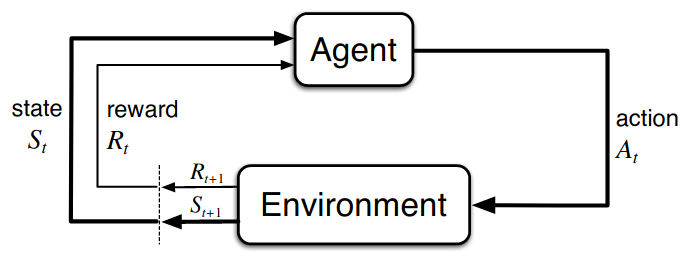
\includegraphics[width=.7\textwidth]{figures/reinforcement_learning.png}
    \caption{Interaction between the agent and the environment in reinforcement learning \cite{Sutton:1998}.}
    \label{fig:reinforcement_learning}
\end{figure}

Figure \ref{fig:reinforcement_learning} shows the interaction between an agent and the environment in a MPD. At time step $t$, the agent finds itself at state $s_t$ and performs an action $a_t$ on the environment. Then, the environment evolves to the next state $s_{t+1}$ where the agent receives the reward $r_{t+1}$. As the learning process continues, the agent and the environment produce a sequence or \textit{trajectory $\tau$} of states, actions and rewards:


\begin{equation}
\tau = s_0, a_0, r_1,s_1, a_1, r_2,s_2, a_2, r_3, ...
\label{eq:transition}
\end{equation}


\subsection{On-policy and off-policy Reinforcement Learning}
\label{subsection:on and off-policy Reinforcement Learning}

One of the objectives of this literature review is to establish a clear definition of the concepts on-policy and off-policy in the field of imitation learning. Before that, in this section we will explain their meaning of these terms in reinforcement learning, a field where they are widely used and well known. To the best of our knowledge, the first mention of the terms on-policy and off-policy in reinforcement learning is found in the book \textit{Introduction to Reinforcement Learning} by \cite{Sutton:1998}.

According to Sutton and Barto, on-policy methods use a a single policy, the same policy that is evaluated or improved, is the one used to generate behavior. On the other hand, off-policy methods use two policies: They evaluate or improve a policy, the target policy, while using a different policy to generate the data, the behavior policy. In this case we say that learning is from data \quotes{off} the target policy, and the overall process is termed off-policy learning. \cite{Sutton:1998}. These definitions are the most accepted and used in reinforcement learning and therefore we will use them as reference further in this review. To better understand the terms, we are going to briefly explore two popular RL algorithms, Q-Learning and SARSA to understand what makes the former off-policy and the later on-policy.

\subsection*{Sarsa and Q-learning}
SARSA and Q-learning are Temporal Difference (TD) algorithms that update the knowledge of the agent at every time step by bootstrapping which means that the update is partly based on other learned estimates, without waiting to know the final outcome \cite{Sutton:1998}. Equation \eqref{eq:TD} shows the general update rule of these TD methods \cite{TD:equation:2019}, here \textit{step size} is equivalent to learning rate.


\begin{equation}
\text{New estimate } \leftarrow \text{ Old estimate }+ \text{ Step size }* \left[\text{ Target - Old estimate} \right]
\label{eq:TD}
\end{equation}

Q-Learning was first introduced by \cite{Watkins:1989} and it is considered an off-policy method because if follows a behaviour policy $\beta$ while evaluating another policy $\pi$. Equation \eqref{eq:Q-learning} shows the update rule for this method where $s_t$ and $a_t$ are the state and action at time step $t$, $R$ is the reward obtained for taking $a_t$ at state $s_t$, $\alpha$ is the step size or learning rate and $\gamma$ is  the discount rate. The term $\max_{a} Q(s_{t+1}, a)$ represents  the best estimated value for the next state $s_{t+1}$ and it is independent of the policy being followed.

\begin{equation}
Q^{\text{new}}(s_t, a_t)  \leftarrow Q(s_t, a_t) + \alpha \left[ R  + \gamma {\max_{a} Q(s_{t+1}, a)} - Q(s_t, a_t)\right]
\label{eq:Q-learning}
\end{equation}


SARSA algorithm was first introduced by \cite{Rummery+Niranjan:1994} with the name \quotes{Modified Connectionist Q-Learning (MCQ-L)} and it was Richard Sutton who suggested, in the same publication of Rummery and Niranjan, the name SARSA, as you need to know State-Action-Reward-State-Action before performing an update.  Unlike Q-learning, the policy that SARSA evaluates, is the same with which it generates samples. Equation \eqref{eq:SARSA} shows its update rule.

\begin{equation}
Q^{\text{new}}(s_t, a_t)  \leftarrow Q(s_t, a_t) + \alpha \left[R+ \gamma  Q(s_{t+1}, a_{t+1}) - Q(s_t, a_t)\right]
\label{eq:SARSA}
\end{equation}
When comparing both updating rules in Equations \eqref{eq:Q-learning} and \ref{eq:SARSA}, we can see that in Q-learning the agent learns the optimal policy by using a greedy policy when updating the Q-value (see the \textit{max} in Equation \eqref{eq:Q-learning}). This is what makes Q-learning off-policy, the fact that it can use a policy for generating behaviour different from the greedy policy with which it updates the Q-values. This is key to understand why Q-learning can make use of the experience replay technique as we will see in Section \ref{subsection:Experience Replay}.



\subsection{Online and Offline} 
\label{subsection:Online and Offline}

Reinforcement learning algorithms can also be classified according to how data is collected. Traditional RL algorithms are active or online frameworks \cite{youtube_offline_RL}, where an agent iteratively interacts in its environment collecting experience and using it to update its policy. Online RL algorithms can be on-policy if  they use data exclusively collected by the current agent, or off-policy, see Table \ref{tab:RL-classification}; some off-policy RL algorithms are able to use previous data but the agent continues interacting with the environment collecting more data that is added to a buffer and then uses the data from the buffer to improve its policy. A remark from the authors of the previous classification is that the algorithm Q-learning is an extreme case where the buffer size is  equal to 1 \cite{Offline-RL-Levine:2020}.

The online approach works well in very specific and  simulated environments however, for real-world settings, online learning is impractical because the agent still needs to collect a diverse and huge data set at each iteration. 

Offline reinforcement learning, see Table \ref{tab:RL-classification}, also called batch RL, data-driven RL or fully off-policy RL,  addresses the aforementioned problem. The key idea is that a large and diverse dataset is previously collected by some behaviour policy and added into a buffer. Then using only that data, the agent has to learn the best possible policy without further interacting with the environment. With this offline framework, it is possible to apply RL to real-world domains like robotics where the agent, the robot, could easily get damaged while collecting data iteratively in an online manner. The downside of offline learning resides in collecting a suitable dataset for training which for many real-world applications, data can be very expensive to acquire \cite{collecting_data_for_offline_learning}.





\begin{table}[]
\begin{tabular}{c|c|l|l|l|}
\cline{2-5}
\textbf{} &
  \multicolumn{2}{p{5cm}|}{\textbf{Only use data collected by current agent}} &
  \multicolumn{2}{c|}{\textbf{Use data collected by other agents}} \\ \hline
\multicolumn{1}{|p{3cm}|}{\textbf{Data collection using current agent}} &

  \multicolumn{2}{l|}{\begin{tabular}[c]{@{}l@{}}
  
Online, on-policy RL \\

  \raisebox{-\totalheight}{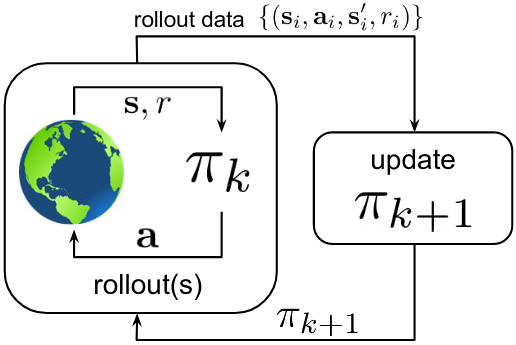
\includegraphics[width=5cm]{figures/on-policy.png}}
  \vspace{5mm} 
  
  \end{tabular}} &
  
  \multicolumn{2}{l|}{\begin{tabular}[c]{@{}l@{}}
  
Online, off-policy RL \\

  \raisebox{-\totalheight}{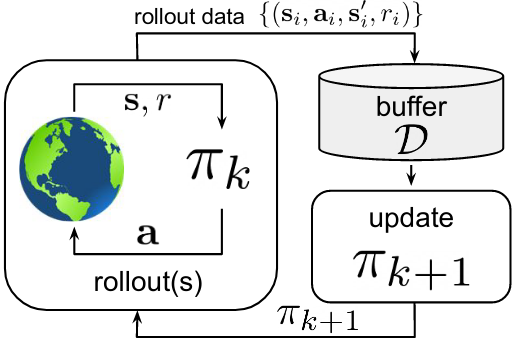
\includegraphics[width=5cm]{figures/off-policy.png}}
  \vspace{5mm} 
  
  \end{tabular}} \\ \hline
  
\multicolumn{1}{|p{3cm}|}{\textbf{Fixed dataset (no additional data collection)}} &
  \multicolumn{2}{c|}
  {-} 
  &
  \multicolumn{2}{l|}{\begin{tabular}[c]{@{}l@{}}
  
  Offline (fully off-policy) RL \\
  
  \raisebox{-\totalheight}{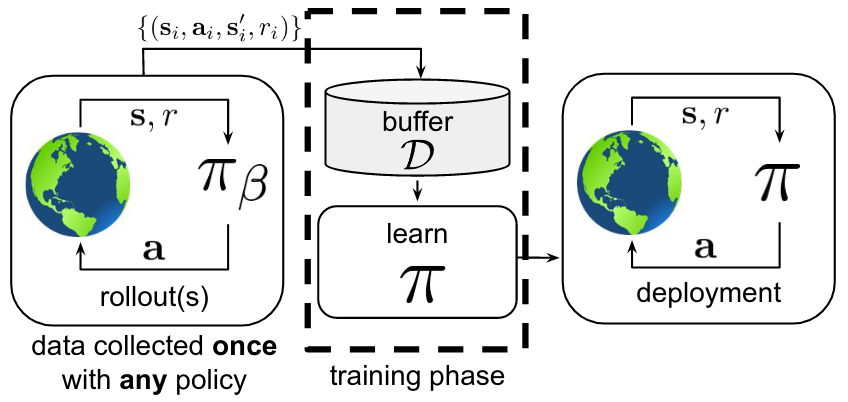
\includegraphics[width=7cm]{figures/offline.png}}
  
  \end{tabular}} \\ \hline
\end{tabular}
\caption{Classification of RL algorithms, \cite{Google_offline_RL}, \cite{youtube_offline_RL}
and \cite{Offline-RL-Levine:2020}.}
\label{tab:RL-classification}
\end{table}











\subsection{Experience Replay}
\label{subsection:Experience Replay}

Experience Replay is a replay memory technique in which the transitions, $<s_t, a_t, r_{t+1}, s_{t+1}>$, gathered by an agent at every time step $t$ are stored into a memory or \textit{replay buffer}. The idea of experience replay is to randomly sample mini-batches of experience from the buffer to update the policy. 



% Three benefits are obtained with this technique: ER is an efficient manner of taking advantage of the experience that has been already collected and use it to learn multiple times \cite{Experience-Replay-zhang:2018}. On the other hand is a way to train the policy with  uncorrelated data  which makes the Neural Network  more robust against locally overfitting to the most recent trajectories, also known as a forgetting phenomenon. 

Experience replay provides several benefits. First, it is an efficient manner of taking advantage of the experience that has been already collected and use it to learn multiple times \cite{Experience-Replay-zhang:2018}. This is particularly important in the case of neural networks because it increases their stability helping to preserve old knowledge and thus reducing catastrophic forgetting \cite{Experience_replay_stability:2019}.
Furthermore, experience replay provides uncorrelated data to train the neural network which helps it to generalize and to minimize overfitting to the most recent trajectories \cite{Machine_learning_finance:2019}.

 

To be able to use this experience replay technique, it is necessary to have an off-policy algorithm. Off-policy RL methods continue estimating the optimal Q-value, $Q^*$, even if the policy that they follow changes from $\pi_1$ to $\pi_2$. However, an on-policy method following a policy $\pi_1$ will yield a Q-value $Q_{\pi_1}$ and if the policy changes to $\pi_2$, it will yield $Q_{\pi_2}$; the optimal Q-value in this last situation wont be guaranteed. It is important to remark that even if the experiences were collected with a single policy $\pi$, because the policy evolves over time, the same policy at time step t, $\pi_t$, is not equal to that same policy in a later time step, $\pi_N$; they are considered experiences gathered by \textit{different policies} and therefore only off-policy methods are applicable.













\section{Imitation Learning}
\label{section:Imitation Learning}

Imitation learning is a problem in machine learning where an agent learns a task leveraging the knowledge of a teacher which can be a human or a more experienced agent \cite{Imitation-Learning-definition-torabi:2019}. Imitation learning is more useful with respect to reinforcement learning when it is easier for a teacher to demonstrate or provide feedback in order for the agent to learn rather than to specify a reward function which would lead to the desired behaviour. The simplest imitation learning algorithm is called behavioural cloning where a teacher provides some initial demonstrations and the agent tries to learn a policy via supervised learning.


\subsubsection{Interactive Imitation Learning}
\label{subsubsection:Interactive-Imitation-Learning}

Interactive imitation learning is a branch of imitation learning \cite{lazydagger:2021}, where the teacher interacts with the agent \textit{during} its training providing feedback to improve its behaviour, see Figure \ref{fig:interactive_imitation_learning}. Some authors \cite{Osa:2018} consider these interactive techniques as a special part of behavioural cloning but to make a more clear distinction it is preferable to consider them as a branch of IL.



\begin{figure}[H]
    \centering
    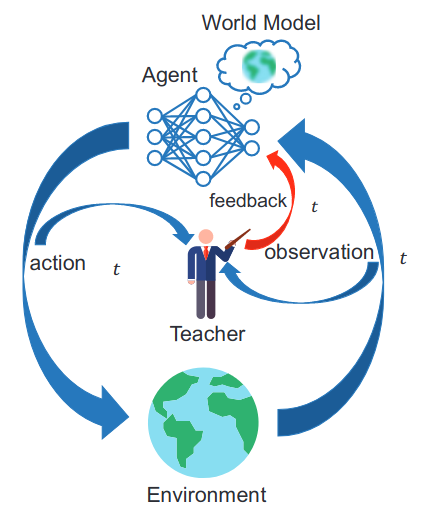
\includegraphics[width=.4\textwidth]{figures/interactive_imitation_learning.png}
    \caption{Interactive Imitation Learning \cite{D-COACH-Dattari-Celemin-Ruiz-del-Solar-Kober:2018}}
    \label{fig:interactive_imitation_learning}
\end{figure}

 The nature of the feedback varies between frameworks: Feedback in the form of evaluations (e.g., the TAMER framework \cite{TAMER-Knox-Stone:2009}) inform the agent how good or bad was the action taken. This kind of evaluative feedback is easier to implement than to define a reward function and allows a faster convergence than pure autonomous learning. 
However, the informativeness of this kind of evaluative feedback is still limited \cite{types-feedback-najar:2020}, and one way to improve it is to use corrections. Feedback as relative corrections \cite{Relative-corrections-Celemin:2019} gives name to corrective imitation learning, a branch of IIL. Corrective feedback improves the informativeness of evaluative feedback, by allowing the teacher to inform the agent whether the value of a taken action should be increased or decreased [Celemin and Ruiz-Del-Solar, 2019]. This requires less exploration compared to evaluative feedback \cite{types-feedback-najar:2020}. Section \ref{section:Corrective Imitation Learning} provides more details about corrective imitation learning.




\subsubsection{On-policy and off-policy Imitation Learning}
\label{subsubsection:on and off-policy Imitation Learning}

Subsection \ref{subsection:on and off-policy Reinforcement Learning} explained the meaning of the terms on-policy and off-policy in the field of reinforcement learning. When researching the literature it is clear that, for RL,  the definition provided by Sutton and Barto in 1998 is the most used. However things are not that obvious when talking about imitation learning. According to the paper \textit{An Algorithmic Perspective on Imitation Learning} \cite{Osa:2018} the first mention to the terms on-policy and off-policy regarding imitation learning is due to \cite{DBLP:journals/corr/LaskeyLHLMFG17}. These definitions are:
\setlength{\parskip}{1em} 

\say{In Off-Policy imitation learning, an agent observes demonstrations from a supervisor and tries to recover the behavior via supervised learning, an example of off-policy IL is behavioral cloning. On-policy imitation learning methods sample trajectories from the agent’s current distribution and update the model based on the data received. A common on-policy algorithm is DAgger.} 

\setlength{\parskip}{1em} 

Similar definitions are found in \cite{OtherLaskeydefinitions:2019} and \cite{Anotherdefinitionfromberkeley:2020}:

\say{On-policy imitation learning involves executing the current agent's policy $\pi_{\theta_i}$ in the environment allowing it to make errors and observe new states and then soliciting feedback from a supervisor on the visited states to update $\pi_{\theta_i}$. This is in contrast to off-policy imitation learning algorithms where policy learning is performed entirely on states from the supervisor's trajectory distribution.}
 
\setlength{\parskip}{1em} 

While we agree with the previous definition of on-policy IL, regarding off-policy IL, we consider that it is easier to interpret and relate its meaning to RL, simply as the opposite of on-policy IL. Therefore our reinterpretation of the definitions is:  

\begin{itemize}
  \item \textbf{On-Policy imitation learning}: \quotes{On-Policy IL methods sample trajectories using the current agent’s policy and use that data to update that same policy.}
  
  \item \textbf{Off-Policy imitation learning}: \quotes{Off-Policy IL methods sample trajectories using a policy different from the current agent’s one.}
  


\end{itemize}

For the case of off-policy imitation learning, the \textit{different policy} could be a combination of different policies including the one of the agent, as it happens in off-policy RL.


In \cite{DBLP:journals/corr/LaskeyLHLMFG17}, \cite{OtherLaskeydefinitions:2019} and \cite{Osa:2018} the first example of on-policy imitation learning given is DAgger (Dataset  Aggregation) \cite{DAgger-Ross:2011}; however, according to their own definitions we consider important to make a clarification regarding this classification. Algorithm \ref{al:DAgger-simplest} shows DAgger's \textit{simplest form}. For the first iteration, DAgger uses the expert’s policy $\pi^*$ (line 2), to collect a dataset of trajectories $D$ and then, it trains a policy  $\hat{\pi}_2$ that best mimics the expert on those trajectories. Then at iteration $n$, it uses $\hat{\pi}_n$ to collect more trajectories and adds those trajectories to the dataset $D$. The next policy $\hat{\pi}_{n+1}$ is the policy that best mimics the expert on the whole dataset $D$. In summary, DAgger uses its \textit{current policy} to collect a dataset at each iteration and trains the next policy under the aggregate of all collected datasets \cite{DAgger-Ross:2011}.

\begin{algorithm}[H]
\caption{Simplest version of DAgger algorithm }
\begin{algorithmic}[1]
\State \textbf{Initialize} $\mathcal{D} \leftarrow 0$ 
\State \textbf{Initialize} $\hat{\pi}_1 \leftarrow \pi^*$ 
\For {$i = 1 $  \textbf{to} $N$} 
\State Let $\pi_i = \hat{\pi}_i$
\State Sample T-step trajectories using $\pi_i$
\State Get dataset  $\mathcal{D}_i = \{(s, \pi^*(s))\}$ of visited states by $\pi_i$ and actions given by expert
\State Aggregate datasets:  $\mathcal{D} \leftarrow \mathcal{D} \cup  \mathcal{D}_i$
\State  Train classifier $\hat{\pi}_{i+1}$ on $\mathcal{D}$
\EndFor
\State Return best $\hat{\pi}_i$ on validation
\end{algorithmic}
\label{al:DAgger-simplest}
\end{algorithm}

This simple version of DAgger fits in the definition of on-policy imitation learning found in the literature because as can be seen in lines 4 and 5 of Algorithm \ref{al:DAgger-simplest}, the policy that gathers the trajectories is the current agent's policy.


However, and to better leverage the knowledge of the expert, the authors \textit{optionally} allow the algorithm to use a modified policy $\pi_i=\beta_i\pi^*+ (1−\beta_i)\hat{\pi}_i$. Depending on $\beta$,  which has values within the range $[0,1]$, the expert policy $\pi^*$, is able to collect part of the next dataset by itself. If $\beta = 1$, the expert has full control when collecting the data as is the case in Behavioural Cloning, opposite to $\beta=0$  which means that all the data is gathered by the current agent's policy. The parameter $\beta$ can be equal to $\beta_i=p^{i−1}$ representing a decaying rate over time of the usage of the expert to collect the data.


This more generic version represented in Algorithm \ref{al:DAgger-general} would not fit into the definition of on-policy imitation learning given by \cite{Osa:2018}, \cite{DBLP:journals/corr/LaskeyLHLMFG17}, \cite{OtherLaskeydefinitions:2019} and \cite{Anotherdefinitionfromberkeley:2020} because the expert's policy  intervenes in collecting the data.



\begin{algorithm}[H]
\caption{DAgger algorithm with stochastic mixing of the agent and the supervisor policies }
\begin{algorithmic}[1]
\State \textbf{Initialize} $\mathcal{D} \leftarrow 0$ 
\State \textbf{Initialize} $\hat{\pi}_1 \leftarrow \pi^*$ 
\For {$i = 1 $  \textbf{to} $N$} 
\State Let $\pi_i = \beta_i\pi^* + (1 -\beta_i)\hat{\pi}_i$
\State Sample T-step trajectories using $\pi_i$
\State Get dataset  $\mathcal{D}_i = \{(s, \pi^*(s))\}$ of visited states by $\pi_i$ and actions given by expert
\State Aggregate datasets:  $\mathcal{D} \leftarrow \mathcal{D} \cup  \mathcal{D}_i$
\State  Train classifier $\hat{\pi}_{i+1}$ on $\mathcal{D}$
\EndFor
\State Return best $\hat{\pi}_i$ on validation
\end{algorithmic}
\label{al:DAgger-general}
\end{algorithm}

To summarize this section, if the teacher intervenes somehow in the actions executed by the agent, we consider this imitation algorithm to be off-policy.

\subsubsection{Imitation Learning algorithms}
\label{subsubsection:Imitation Learning algorithms}

In this section, we gather and briefly describe some Imitation Learning algorithms with the objective of later classify them according to the proposed definitions from the previous subsection.




\subsubsection*{Behavioural Cloning}
Behavioural cloning (BC) \cite{Behavioural-Cloning-Pomerleau:1991}, one of the oldest Imitation Learning frameworks, consists on directly learning a policy, via supervised learning, given a data set of demonstrations provided by a teacher. The main problem with BC is known as \textit{distribution mismatch} and it happens because at the moment that the learner agent deviates from the expert trajectory, it cannot recover from that failure and go back to the expert trajectory. This provokes a cascade of errors that keep growing because the agent does not know how to act in those states that have not been visited by the expert \cite{Global-overview-Attia:2018}.

\subsubsection*{Inverse Reinforcement Learning methods}
Inverse Reinforcement Learning (IRL) is two-step approach for learning from humans. First, based on demonstrations provided by the human expert, the agent learns the reward function $R$ that best explains the behaviour of the human. Then, with this reward function, the optimal policy is learnt using RL methods \cite{inverse-reinforcement-learning}.

\subsubsection*{Learning from human preferences methods}
Learning from human preferences, \cite{learning-from-human-preferences:2017}, \cite{learning-from-human-preferences:2018},  are methods where iteratively, a human decides which of several executions of a policy is better according to the goal of the task. Then, a reward function that explains the decisions of the human is found and with it and applying RL, the agent learns how to perform the task. The user continues deciding between executions and so,  the policy gradually improves.


\subsubsection*{DART}
DART (Disturbances for Augmenting Robot Trajectories) \cite{DART-Laskey:2017} is an algorithm close to behavioural cloning \cite{Behavioural-Cloning-Pomerleau:1991}. According to its authors is an off-policy imitation learning algorithm because, after the first expert's demonstration, it does not require to query the expert anymore. This method works by injecting noise into the supervisor's policy while demonstrating the task, in order to force visiting a wider region of the state space and get the recovery demonstrations, therefore reducing the problem of distribution mismatch.

\subsubsection*{SQIL}
SQIL (Soft Q Imitation Learning) \cite{SQIL-Reddy-Dragan-Levine:2019} is a variant of behavioural cloning that incentives the agent to match human demonstrations over a long horizon. SQIL uses reinforcement learning but does not learn a reward function, instead, when the agent matches a demonstrated action in a demonstrated state, it receives a reward of "1" and "0" for every other behaviour.

\subsubsection*{ValueDICE}
ValueDICE (Distribution Correction Estimation) \cite{ValueDICE-Kostrikov:2019}, is an off-policy imitation learning \cite{Laskey:phdthesis} that minimize the KL-divergence between the expert distribution and the distribution induced by the agent when interacting with the environment in a off-policy manner.

%% DAGGERS!%%%%%%%%%%%%%%%%%%%

\subsubsection*{DAgger}
DAgger (Data Aggregation) \cite{DAgger-Ross:2011} is one of the most well-known imitation learning algorithms and it was explained in-depth in Section \ref{subsubsection:on and off-policy Imitation Learning}. Many variants of DAgger exist and some of them are going to be commented on next.



\subsubsection*{DAgger by coaching}
DAgger by coaching \cite{DAgger-by-coaching-He-DaumeIII-Eisner:2012},  is a version of DAgger \cite{DAgger-Ross:2011} where the human teacher executes actions that are within learner’s ability. This means that when the agent is at a state far from the desired state, the teacher will not try to correct directly that difference but instead it will try to redirect the agent gradually \cite{Global-overview-Attia:2018}.


\subsubsection*{AggreVaTe}
AggreVaTe (Aggregate Values to Imitate) \cite{AggreVaTe-Ross-Bagnell:2014}, is a version of DAgger \cite{DAgger-Ross:2011}, that learns to choose actions that minimize the cost-to-go of the expert, 
\cite{Global-overview-Attia:2018}. The cost-to-go $Q$ is the cost of executing an action in a state and continue executing a policy for the next steps. The first iteration is the same as in DAgger, then for the next iterations,  at a time t, the cost-to-go $Q$ of taking an action in a state is observed and added to the the initial dataset $D$ together with the action and the state.



\subsubsection*{AggreVaTeD}
AggreVaTeD \cite{AggreVaTeD-Sun:2017} is a differentiable version of the AggreVaTe algorithm introduced by \cite{AggreVaTe-Ross-Bagnell:2014} that does not perform any data aggregation. It includes two gradient update procedures: An online gradient descent and a natural gradient update similar to exponential gradient descent.

\subsubsection*{SafeDAgger}
SafeDAgger \cite{SafeDAgger-Zhang-Cho:2016}, is a version of DAgger \cite{DAgger-Ross:2011}, that aims to reduce the burden of constantly querying the human teacher by incorporating a safety policy. This safety policy predicts the discrepancy between the teacher and the learner and it is only on those states where the discrepancy is high, that the teacher is queried.


\subsubsection*{DropoutDAgger}
DropoutDAgger \cite{DropoutDAgger} is a method similar to SafeDAgger \cite{SafeDAgger-Zhang-Cho:2016}. It uses the dropout technique to train the neural network policy applying $N$ random dropout masks. For each random configuration of the network, an action is obtained for the same input observation. Only if its distribution over actions has enough probability mass around the action suggested by the expert, the mean action of the novice is taken, otherwise the action of the expert is chosen. When the distribution of actions has high entropy it means that that region of the state-space is unfamiliar and therefore, it is safer to chose the action of the expert.

\subsubsection*{EnsembleDAgger}
EnsembleDAgger \cite{EnsembleDAgger-Menda:2019}, is an extension of DAgger where the learning agent only acts when two measures are compliant with two preset thresholds: The first measure is the \textit{discrepancy}, which is the same as in SafeDagger \cite{SafeDAgger-Zhang-Cho:2016}; discrepancy represents the deviation between the agent and the expert. The second measure is the \textit{doubt} which is the variance that indicates the familiarity of the agent with its current state; the doubt constrains the learner to only act in familiar states. 

\subsubsection*{ThriftyDAgger}
ThriftyDAgger \cite{ThriftyDAgger} is a method similar to SafeDagger \cite{SafeDAgger-Zhang-Cho:2016} and EnsembleDAgger \cite{EnsembleDAgger-Menda:2019} in the sense that it switches the control between the agent and the human supervisor depending on the novelty and the risk of a particular state. ThriftyDAgger proposes a novel metric for measuring the riskiness of a state which captures the likelihood that the agent cannot succeed in converging to the goal state.

\subsubsection*{SHIV}
SHIV (Svm-based reduction in Human InterVention) \cite{SHIV-Laskey:2016},  is a method similar to DAgger \cite{DAgger-Ross:2011} that differs from this one in the fact that the human teacher is not queried to provide labels for all the visited states but only when it is risky. The risk is described as distance to a boundary defined by a one class support vector machine.

\subsubsection*{Hierarchical Guidance DAgger}
Hierarchical guidance \cite{Hierarchical-guidance-Le:2018} is a framework for hierarchical problems where low level sub-tasks can be identified by an expert. The authors present two settings: In the first one, hierarchical imitation learning,  the teacher provides high-level feedback and only provides low-level feedback when needed. The second setting is a hybrid imitation–reinforcement learning where the teacher provides only high-level feedback and the learner uses reinforcement learning at the low level.



\subsubsection*{BAgger}
BAgger (Bayesian  dataset  Aggregation) \cite{BAgger-Cronrath:2018}, is an extension of DAgger \cite{DAgger-Ross:2011} that aims to increase safety and reduce expert burden by querying the expert only when there is risk of not being able to imitate the expert. BAgger trains a Bayesian neural network or a Gaussian process to predict the expected error between teacher and learner.


















\subsubsection*{SAIL}
SAIL (Safety-Aware Imitation Learning) \cite{SAIL-Xiong:2019}, is an extension of DAgger that aims to reduce the number of queries to the expert. Only when the confidence level of the learning agent is lower than a threshold, is the expert queried. The expert continues providing labels until the confidence in all states is again higher than a threshold. Then, an uncertainty based approach decides whether or not continue querying the expert.

\subsubsection*{Retrospective DAgger}
Retrospective DAgger \cite{Retrospective-DAgger-song:2019}, is a version of the DAgger \cite{DAgger-Ross:2011} algorithm, designed for combinatorial search spaces. The policy learns from its mistakes by learning from retrospective inspections of its own roll-outs.  

\subsubsection*{HG-DAgger}
HG-DAgger (Human-Gated Data Aggregation) \cite{HG-DAgger-Kelly:2019}, is a version of DAgger \cite{DAgger-Ross:2011} that includes a gating function controlled by the expert; when the expert teacher detects that the agent is at a unsafe region of the state space, the expert takes control and leads the learning agent to a safe region of the state space.

\subsubsection*{EIL}
EIL (Expert Intervention Learning) \cite{EIL-Spencer:2020}, is an algorithm similar to HG-Dagger, that allows the teacher to take the control of the agent when needed. In HG-Dagger,  the labels that the human provides when taking control (explicit feedback) are used to update the data set. On the other hand, EIL not only uses this explicit feedback but also the implicit feedback which are those actions that the human does not correct because the agent is already behaving correctly. Finally, EIL also takes into account the timing, meaning when the feedback was provided.

\subsubsection*{FIRE}
FIRE (Failure Identification to Reduce Expert burden) \cite{FIRE-ablett:2020}, is an algorithm similar to HG-Dagger that incorporates the ability of notifying the expert when the agent is at a unsafe state. FIRE has a  failure predictor that classifies expert and non-expert data and predicts when a failure may occur. When this happens, the policy stops and if the human agrees with the prediction, he/she teleoperates the agent back to a safe state.

\subsubsection*{IWR}
IWR (Intervention Weighted Regression) \cite{IWR-mandlekar:2020} is an algorithm similar to FIRE, that focuses on \textit{bottlenecks} regions, that is, those states where it is necessary a sequence of precise actions. IWR keeps two different data sets, one with data provided by the human when intervening in a trajectory (mostly during bottleneck regions), and another one for the rest of the trajectory when the human does not intervene. During training, the two data sets are equally sampled which re-weights  the data distribution to reinforce those labels provided by the human  during bottleneck regions, while the data sampled from the non-intervention data set
keeps the policy close to previous policy iterations \cite{IWR-mandlekar:2020} .



\subsubsection*{DA-RB}
DA-RB (DAgger Replay Buffer) \cite{DA-RB-Prakash:2020}, is an extension of the DAgger algorithm \cite{DAgger-Ross:2011} that incorporate an additional replay buffer with the aim of controlling, in the data set, the proportion of data provided by the human and data gathered by the agent. This buffer is said to help the policy to focus on its weaker behaviours.




 
 \subsubsection*{COACH}
COACH (COrrective Advice Communicated by Humans) \cite{COACH-Celemin-Ruiz-del-Solar:2015}, is an algorithm designed for non-expert humans where feedback is provided as a binary signal interpreted as an increase or decrease of the value of an action.  The feedback is immediately used for updating the policy which makes it easy for the teacher to observe the change in the behaviour of the agent and continue providing further corrections. When a sequence of corrections has the same sign, it indicates that the correction to be made has a large magnitude. Opposite, if the signal alternates signs, the teacher is trying to make smaller corrections around a certain state. Furthermore, COACH includes a Human Feedback Model that helps to interpret and adapt the corrections.
This algorithm, and more specifically its deep version \cite{D-COACH-Dattari-Celemin-Ruiz-del-Solar-Kober:2018} are the main focus of this master thesis.

\subsubsection*{D-COACH}
D-COACH (Deep COrrective Advice Communicated by Humans) \cite{D-COACH-Dattari-Celemin-Ruiz-del-Solar-Kober:2018} is the deep learning version of the COACH algorithm \cite{COACH-Celemin-Ruiz-del-Solar:2015}. It uses artificial neural networks to represent the policy and includes a buffer to replay recent experiences. As already mentioned, this algorithm is the starting point of the present master thesis.



\subsubsection*{Advise}
Advise \cite{Advise-Griffith-et-al:2013}, is a policy shaping approach where the human teacher feedback is interpreted as direct policy labels; example of feedback could be \say{this is right} or \say{this is wrong} given an action taken by the agent. Advise also takes into account that the human feedback can be inconsistent and that correct feedback is provided with a probability $C$. Advise uses this probability and the Bayes rule to represent the human feedback policy \cite{leveraging-human-guidance:2019}.

\subsubsection*{I-SABL}
I-SABL (Inferring Strategy-Aware Bayesian Learning) \cite{I-SABL-Loftin:2016}, which is most similar to Advise \cite{Advise-Griffith-et-al:2013} uses expectation-maximization to calculate the best action. With this method, if the learning agent takes an optimal action, the human teacher provides positive feedback, otherwise, the human provides negative feedback \cite{leveraging-human-guidance:2019}.


\subsubsection*{ABLUF}
ABLUF (Adaptive Bayesian Learning with Uncertain Feedback) \cite{ABLUF-he:2020}, is based on expectation maximization algorithms, and it is similar to I-SABL \cite{I-SABL-Loftin:2016}. However, whereas I-SABL assumes that the expert only provides positive feedback when the agent takes an optimal action, ABLUF models the human feedback as a probability distribution, where the probability of providing positive or negative feedback, increases or decreases with respect to the distance between the action taken and the optimal action.



\subsubsection*{TAMER}
In the TAMER (Training an Agent Manually via Evaluative Reinforcement) framework \cite{TAMER-Knox-Stone:2009}, the teacher is seen as a reward function that maps the actions of the agent to negative, neutral or positive feedback. This kind of feedback is called evaluative feedback because the teacher evaluates how good or bad is the action taken by the agent. This reward function replaces the rewards provided by the environment in a classical reinforcement learning problem \cite{leveraging-human-guidance:2019}.
 

\subsubsection*{Deep TAMER}
Deep TAMER \cite{DeepTAMER-Warnell-et-al:2018} is a version of the TAMER framework \cite{TAMER-Knox-Stone:2009} where the policy is represented with a deep neural network.

\subsubsection*{DQN-TAMER}
DQN-TAMER \cite{DQN-TAMER-Arakawa:2018}, is a combination of the TAMER framework \cite{TAMER-Knox-Stone:2009} with Deep Q-Network (DQN). The original TAMER framework does not take into account the environment reward, but DQN-TAMER trains a DQN agent and a TAMER agent, and the final decision policy is a weighted average of the policies from both agents \cite{leveraging-human-guidance:2019}.

\subsubsection*{Convergent Actor-Critic by Humans}
Convergent Actor-Critic by Humans \cite{fakeCOACH-MacGlashan-Ho-Loftin:2017}, is an algorithm inspired in TAMER \cite{TAMER-Knox-Stone:2009} that differs from this one in that fact that TAMER interprets human feedback as a reward function independent of the agent’s current policy \cite{leveraging-human-guidance:2019}. 
Contrary, Convergent Actor-Critic by Humans assumes that human feedback depends on the agent's current policy and that it should be interpreted as the advantage function that tells how much better or worse when deviating from the agent’s current policy.

\subsubsection*{FRESH}
FRESH (Feedback-based REward SHaping) \cite{FRESH-xiao:2020}, is similar to Deep-TAMER \cite{DeepTAMER-Warnell-et-al:2018} but unlike Deep-TAMER, FRESH takes into account the reward from the environment.



\subsubsection*{LOKI}
LOKI (Locally Optimal search after K-step Imitation) \cite{LOKI-Cheng:2018}, is an algorithm that has two phases: A first imitation learning phase and a second reinforcement learning phase. First, it randomly picks a number within a range and performs that number of online imitation learning steps. Then, in the reinforcement learning phase, it improves the policy with a policy gradient RL method.










\subsubsection*{AOR}
AOR (Adaptive On-Policy Regularization) \cite{AOR-lee-laskey:2019}, is an algorithm that uses dynamic regret which measures performance of a policy at each iteration. Dynamic regret compares the current  policy  against  the  best  it  could  be  on  its  distribution with  respect  to  the  expert \cite{Dynamic-regret-Laskey:2018}.  

















\subsubsection*{Cycle-of-Learning}
Cycle-of-Learning \cite{Cycle-of-Learning-waytowich:2018},  is a framework that allows to switch between multiple types of human interventions when teaching an agent. Human interactions are divided in three categories arranged from more human control to less human control: Learning from human demonstration, learning from human intervention and learning from human evaluation. As the learning task progresses in time and the agent improves, less human intervention is required and therefore the algorithm switches to the following type of intervention technique.


\subsubsection{Classification of Imitation Learning algorithms as on-policy or off-policy}
\label{subsubsection:Classification of Imitation Learning algorithms as on-policy or off-policy}

Table \ref{tab:classification_table} shows the classification of the previous imitation learning algorithms according to the definitions shown in Section \ref{subsubsection:on and off-policy Imitation Learning}.

\begin{table}[H]
\begin{tabular}{c|c|l|l|l|}
\cline{2-5}
\textbf{} &
  \multicolumn{2}{p{6.5cm}|}{\vspace{0.5mm} \textbf{On-policy Imitation Learning}\vspace{0.5mm}} &
  \multicolumn{2}{p{6.5cm}|}{\vspace{0.5mm}\textbf{Off-policy Imitation Learning}} \\ \hline
\multicolumn{1}{|p{1.8cm}|}{\textbf{Online IL}\vspace{0.5mm}} &

  \multicolumn{2}{p{6.5cm}|}{\begin{tabular}[c]{@{}l@{}}

  \vspace{1mm} \\
  TAMER \hspace{1mm} \cite{TAMER-Knox-Stone:2009}\\ 


  COACH \hspace{1mm}\cite{COACH-Celemin-Ruiz-del-Solar:2015}\\ 
  SHIV \hspace{1mm} \cite{SHIV-Laskey:2016}\\ 
  I-SABL \hspace{1mm}\cite{I-SABL-Loftin:2016}\\
  Convergent Actor-Critic by Humans \hspace{1mm}\cite{fakeCOACH-MacGlashan-Ho-Loftin:2017}\\
  Deep TAMER \hspace{1mm}\cite{DeepTAMER-Warnell-et-al:2018}\\ 
  D-COACH \hspace{1mm}\cite{D-COACH-Dattari-Celemin-Ruiz-del-Solar-Kober:2018}\\ 
  DQN-TAMER \hspace{1mm}\cite{DQN-TAMER-Arakawa:2018}\\
  LOKI \hspace{1mm}\cite{LOKI-Cheng:2018}\\
  AOR \hspace{1mm}\cite{OtherLaskeydefinitions:2019}\\
  ABLUF \hspace{1mm}\cite{ABLUF-he:2020}\\
  EIL \hspace{1mm}\cite{EIL-Spencer:2020}\\
    Learning from human preferences
  \cite{learning-from-human-preferences:2018}\\
\vspace{1mm} \\

  \end{tabular}} &
  
  
  
  
  \multicolumn{2}{l|}{\begin{tabular}[c]{@{}l@{}}
  \vspace{1mm} \\
  DAgger\hspace{1mm}\cite{DAgger-Ross:2011} \\
  DAgger by coaching \hspace{1mm} \cite{DAgger-by-coaching-He-DaumeIII-Eisner:2012}\\
  Advise \cite{Advise-Griffith-et-al:2013}\\
  AggreVaTe \hspace{1mm} \cite{AggreVaTe-Ross-Bagnell:2014}\\ 
  Safe DAgger \hspace{1mm} \cite{SafeDAgger-Zhang-Cho:2016}\\ 
  DropoutDAgger \hspace{1mm} \cite{DropoutDAgger}\\ 
  AggreVaTeD \hspace{1mm}\cite{AggreVaTeD-Sun:2017}\\
    Hierarchically Guided DAgger \hspace{1mm}\cite{Hierarchical-guidance-Le:2018}\\
  BAgger \hspace{1mm}\cite{BAgger-Cronrath:2018}\\ 
  Cycle of Learning \hspace{1mm}\cite{Cycle-of-Learning-waytowich:2018}\\
  Retrospective DAgger \hspace{1mm}\cite{Retrospective-DAgger-song:2019}\\ 
  SAIL \hspace{1mm}\cite{SAIL-Xiong:2019}\\
  HG-DAgger \hspace{1mm}\cite{HG-DAgger-Kelly:2019}\\
  EnsembleDAgger \hspace{1mm}\cite{EnsembleDAgger-Menda:2019}\\
  DAgger Replay Buffer \hspace{1mm}\cite{DA-RB-Prakash:2020}\\
  FRESH \hspace{1mm}\cite{FRESH-xiao:2020}\\
  FIRE \hspace{1mm}\cite{FIRE-ablett:2020}\\
  IWR \hspace{1mm}\cite{IWR-mandlekar:2020}\\
  ThriftyDAgger \hspace{1mm}\cite{ThriftyDAgger}

\vspace{1mm} \\





  
  
  \end{tabular}} \\ \hline
  
\multicolumn{1}{|p{1.8cm}|}{\textbf{Offline IL}} &
  \multicolumn{2}{c|}
  {-} 
  &
  \multicolumn{2}{l|}{\begin{tabular}[c]{@{}l@{}}
  \vspace{1mm} \\
  
  Behavioural Cloning \hspace{1mm}\cite{Behavioural-Cloning-Pomerleau:1991}\\ 
  DART \hspace{1mm}\cite{DART-Laskey:2017}\\ 
  ValueDICE \hspace{1mm}\cite{ValueDICE-Kostrikov:2019}\\
  SQIL \hspace{1mm}\cite{SQIL-Reddy-Dragan-Levine:2019}\\
%   Inverse Reinforcement Learning \hspace{1mm}\cite{inverse-reinforcement-learning}\\
  \vspace{1mm}
  \end{tabular}} \\ \hline
\end{tabular}
\caption{Classification of Imitation Learning algorithms}
\label{tab:classification_table}
\end{table}





\section{Corrective Imitation Learning}
\label{section:Corrective Imitation Learning}


Section 4 concludes this review by explaining in detail the objective of this master thesis and the proposal to carry it out. 
The goal is to transform the corrective imitation learning algorithm D-COACH, which is the deep version of the COACH algorithm, into an off-policy version that will incorporate an improved experience replay without the restrictions present in current version of D-COACH.





As it was presented in Subsection \ref{subsubsection:Interactive-Imitation-Learning}, there are different types of feedback that a teacher can provide during an interactive imitation learning training session. In this Master Thesis we are going to focus on feedback in the form of relative corrections which is the type of feedback used in D-COACH \cite{D-COACH-Dattari-Celemin-Ruiz-del-Solar-Kober:2018}. The usage of corrective feedback names the term corrective imitation learning which we consider as a branch of IIL.


\subsection{COACH: Corrective Advice Communicated by Humans}
\label{subsection:COACH}

COACH \cite{COACH-Celemin-Ruiz-del-Solar:2015} is a CIL framework designed for non-expert humans teachers where the person supervising the learning agent, provides occasional corrections when the agent behaves wrongly. This corrective feedback $h$ is a binary signal that indicates the direction in which the executed action $a = \pi_\theta(s)$, should be modified.
The parameters of the policy $\pi_\theta(s)$, $\theta$ are updated using a stochastic gradient descent (SGD) stategy in a supervised learning manner where the cost function $J(\theta)$ is the mean squared error between the applied and the desired action \cite{Gaussian-COACH-wout:2019}. Equation \eqref{eq:first-update-rule-D-COACH} shows the general update rule of the parameters $\theta$:


\begin{equation}
\theta \leftarrow \theta - \alpha \cdot \nabla_\theta J(\theta)
\label{eq:first-update-rule-D-COACH}
\end{equation}

COACH works under the assumption that teachers are non-experts and that therefore they are just able to provide a correction trend that tells the sign of the policy error but not the error itself. To compute the exact magnitude of the error, COACH incorporates a hyperparameter $e$ that needs to be defined beforehand, resulting in $\text{error}_t = h_t \cdot e$  \cite{COACH-Celemin-Ruiz-del-Solar:2015}. The error needs to be defined as a function of the parameters in order to compute the gradient in the parameter space of the policy; thus, the error can be also described as the difference between the desired action generated with the teacher's feedback, $a^\text{target}_t = a_t + \text{error}_t$ , and $a_t$ is the current output of the policy, $a_t = \pi_\theta(o_t)$:


\begin{equation}
\text{error}_t(\theta) = a_t^\text{target} - a_t
\label{eq:error-D-COACH}
\end{equation}


Equation \eqref{eq:second-update-rule-D-COACH} shows the final update rule of COACH obtained from Equations \eqref{eq:first-update-rule-D-COACH}, \eqref{eq:error-D-COACH} and the derivative of the mean squared error:


\begin{equation}
\theta \leftarrow \theta + \alpha \cdot \text{error}_t \cdot \nabla_\theta \pi_\theta
\label{eq:second-update-rule-D-COACH}
\end{equation}



Where $\nabla_\theta \pi_\theta$ is the gradient of the policy, $\frac{\partial \pi}{\partial \theta}$, w.r.t the parameters $\theta$. Algorithm \ref{al:COACH} shows the pseudocode of the basic COACH version:


\begin{algorithm}[H]
\caption{Basic COACH}
\begin{algorithmic}[1]
\State $e \leftarrow \text{error magnitude}$ 
\State $\alpha \leftarrow \text{learning rate}$ 
\While {$\text{\textit{true}}$} {}
\State $s \leftarrow \text{getStateVec()}$
\State \textbf{execute} action $a_{t}=\pi_{\theta}(s_{t})$
\State \textbf{feedback} human corrective advice $h_{t}$
\If{$h_{t}$ is not \textbf{0}}
\State $\text{error}_{t} = h_{t}\cdot e$
\State $a_{\text{target}(t)} = a_{t} + \text{error}_{t}$
\State \textbf{update} $\pi$ using SGD with pair ($o_{t}$, $a^{\text{target}}_{t}$)
\EndIf
\EndWhile
\end{algorithmic}
\label{al:COACH}
\end{algorithm}

\subsection{D-COACH: Deep COACH}
\label{subsection:D-COACH}


D-COACH \cite{ResearchAssignmentpaper} is the \quotes{deep} version of the COACH algorithm which represents the policy with an Artificial Neural Network.

\begin{algorithm}[H]
\caption{Deep COACH}\label{algorithm:DeepCOACH}
\begin{algorithmic}[1]
\State \textbf{Require:} error magnitude $e$, buffer update interval $b$
\State \textbf{Init:} $\mathcal{B} = [\quad]$  \emph{\# initialize memory buffer}
\For{t = 1,2,...}{}
\State \textbf{observe} state $o_{t}$
\State \textbf{execute} action $a_{t}=\pi_{\theta}(o_{t})$
\State \textbf{feedback} human corrective advice $h_{t}$
\If{$h_{t}$ is not \textbf{0}}
\State $\text{error}_{t} = h_{t}\cdot e$
\State $a_{\text{target}(t)} = a_{t} + \text{error}_{t}$
\State \textbf{update} $\pi$ using SGD with pair ($o_{t}$, $a^{\text{target}}_{t}$)
\State \textbf{update} $\pi$ using SGD with a mini-batch sampled from $\mathcal{B}$
\State \textbf{append} $(o_{t}, a^{\text{target}}_{t})$ to $\mathcal{B}$
\EndIf
\If{mod(t, b) is 0 }
\State \textbf{update} $\pi_{\theta}$ using SGD with a mini-batch sampled from $\mathcal{B}$
\EndIf
\EndFor
\end{algorithmic}
\label{al:D-COACH}
\end{algorithm}

\begin{figure}[H]
    \centering
    \adjustbox{trim=0cm 2cm 0cm 0cm}{%
  \includesvg[width=.9\textwidth]{figures/DCOACH-diagram.svg}}
    \caption{D-COACH agent}
    \label{fig:DCOACH_diagram}
\end{figure}

The current version of D-COACH already implements experience replay to be more data efficient and it does this by incorporating a memory buffer $\mathcal{B}$ (see Algorithm \ref{al:D-COACH}) which the basic version of COACH lacks. During learning, tuples of recent corrections, $(o_t, a^{\text{target}}_t)$, are stored in said memory buffer and then they are replayed. In Section \ref{subsection:Experience Replay} it was mentioned that ER requires off-policy algorithms to work properly, but current D-COACH is on-policy because the policy is updated with data that depends on its most recent version. In this case, the replay buffer $\mathcal{B}$ works by assuming that \textit{recent} feedback is still being valid to update the most recent version of the policy. Due to this assumption, the size of the buffer that D-COACH implements needs to be drastically reduced in comparison with normal ER buffers, otherwise old corrections could update the policy in undesired directions of the policy’s parameter space. On the other hand, a very small ER buffer will provoke an  overfitting of the policy to data generated in the most recent trajectories, which limits the current version of D-COACH to work in short horizon problems.


% However, it is important to remark that this replay buffer $\mathcal{B}$ is not completely correct; as it was mentioned in section \ref{sec:experience-replay}, ER techniques require an off-policy algorithm to work properly, but current D-COACH is on-policy because the policy is updated with data that depends on its most recent version. 



\chapter{Batch Deep COACH (BD-COACH)}
\label{chapter:Proposed Method}

In this chapter we address the question of how a corrective deep imitation learning algorithm can truly leverage old collected corrections. The current version of the CIL algorithm D-COACH is limited to problems that do not require large amounts of data as its replay buffer needs to be kept small. A new method is therefore needed to maximise the full potential of the replay buffer which will allow to train for tasks that are more data demanding. In this chapter we present the method Batch Deep COACH (BD-COACH) an extension of D-COACH that is able to perform policy dependent updates by incorporating a  human model module that learns the feedback from the teacher.

Section \ref{section:Difference between D-COACH and BD-COACH} focuses on the difference between D-COACH and BD-COACH.

Section \ref{section:Proposed method: BD-COACH} explains the modules of the BD-COACH framework.


Finally, section \ref{section:Algorithm-Discussion} gathers the conclusions about the new proposed method.  


\section{Difference between D-COACH and BD-COACH}
\label{section:Difference between D-COACH and BD-COACH}

To mitigate catastrophic forgetting and overfitting, D-COACH makes use of a replay buffer whose size is kept small to avoid old contradictory corrections to be conveyed to the current version of the policy for its update. This limitation makes D-COACH perform worse when facing tasks that require a lot of data and thus, it is limited to the type of problems it can address. There are several aspects that determine the complexity of a task and therefore, the amount of data required for training it. On the one hand, there are problems related to the observation itself, such as how complex it is, or its dimensionality; the higher the dimensionality of the observation, the more difficult the problem is. One way to mitigate the problem of high-dimensional observations such as images is to employ state representation learning (SRL) strategies for learning a low dimensional representation of the state, as D-COACH does. The horizon of the task also has a great impact, the longer the horizon, the more data is required. Finally, another important aspect is the complexity of the decision space of the task. Therefore, a task with a combination of a complex and high-dimensional observation space plus a long horizon and a complex observation-action mapping, would be very challenging for D-COACH to learn.





In D-COACH, batch updates are independent of the policy as corrections from the buffer do not depend on what the policy is currently doing at those particular states. This fact makes that feedback gathered by older versions of the policy can deteriorate the performance of the current policy. If we want to correctly implement the corrections replay technique, we need to answer the following question: How can corrections gathered by older versions of the policy and which are stored in a replay buffer still useful for batch updating the current version of the policy? Remark that this question addresses the \textit{batch update} and not the single update which will be done in the same way as in D-COACH. We need corrections that \textit{depend} on the current agent's policy instead of using corrections gathered by older policies, as happens in D-COACH. This is exactly what the human teacher does and what we want to imitate. The human observes the state and the action of the agent at a particular moment and gives a correction accordingly. We introduce a human teacher learner module in our framework as an artificial neural network that takes pairs of state/actions and outputs the appropriate feedback correction. This module, called the human model, is learned in parallel together with the policy. At the beginning of the training the corrections predicted by the human model will be inadequate, but we expect that, as the training progresses and the human model improves, the predicted corrections will also improve.


We coin this new method Batch Deep COACH (BD-COACH), a CIL framework with policy dependent batch updates. BD-COACH is able to work with higher demanding data tasks thanks to the human model module that learns to predict the feedback that the teacher provides. These predicted corrections depend on the output of the policy at a particular state making them convenient for updating the current version of the policy.


               

\begin{table}[H]
\centering
\renewcommand{\arraystretch}{1.4}
\begin{tabular}{lS[table-format=4]
                 lS[table-format=4]
                 lS[table-format=4]}
\toprule
Method  & {Feedback is:} & {Batch updates are:}\\[-.4em]
\midrule
\textbf{D-COACH}  &   {Policy dependent} &   {Policy independent}\\
\textbf{BD-COACH}  &  {Policy dependent} &   {Policy dependent}\\
\bottomrule
\end{tabular}
\caption{Difference between D-COACH and BD-COACH}
\label{tab:difference-DCOACH-RCIDL}
\end{table}




Table \ref{tab:difference-DCOACH-RCIDL} shows a summary of the dependencies. Notice that for both methods, corrections are always dependent of the policy as the human teacher provides corrections depending on what the policy is doing. What changes between D-COACH and BD-COACH is the dependency of the corrections during the batch updates.



\section{Learning Framework}
\label{section:Proposed method: BD-COACH}

Figure \ref{fig:BD-COACH} depicts the modules that compose the proposed method BD-COACH. The coloured arrows other than black identify the different updates of the policy and the human model. Specifically, the red arrows show the flow of information for a single update of the policy while the green ones are used for representing its batch update. Finally, the blue arrows indicate a batch update of the human model.



\begin{figure}[H]
    \centering
    \adjustbox{trim=0cm 0.3cm 0cm 0.2cm}{%
  \includesvg[width=.86\textwidth]{figures/BD-COACH3.svg}}
    \caption{Modules of the BD-COACH framework}
    \label{fig:BD-COACH}
\end{figure}


\subsection*{Policy}

The policy $\pi(s)$ is the core of the agent that makes decisions in an environment. This function, represented in BD-COACH by an artificial neural network, observes the state of the environment and emits an action accordingly. The policy is learnt during training with both single and batch updates. 


\subsection*{Replay Buffer}
The replay buffer $\mathcal{D}$ is an artificial memory  used to store the experience gathered by the policy on the time steps when the human teacher provides corrections. This information consists on a 3-tuple formed by the state of the environment at time step $t$,  $s_t$, the correspondent action from the policy, $a_t$ and the feedback signal from the human, $h_t$. 

\subsection*{Policy Update Module}
This module, which is the same as in D-COACH, is in charge of updating the policy with both single updates (red loop of Figure \ref{fig:BD-COACH}) and batch updates (green loop of Figure \ref{fig:BD-COACH}). The difference lies in the origin of the information that the module takes as input during the batch update. The corrections that are fed to the policy update module depend on the actions taken by the policy for those states. These corrections do not come directly from the replay buffer as in the case of D-COACH but instead are the output of the human model module.


% Is in this batch update where the main difference with D-COACH can be observed as the batch of corrections that enter the policy update module depend on the actions taken by the policy for those states.

% Single updates happen when at a particular time step during the training, the human teacher considers that the action emitted by the policy, $\pi(s) = a$, should be modified, and provides a feedback signal $h$ to correct the action in the desired direction. This signal is fed directly to the policy update module (red arrow of Figure \ref{fig:BD-COACH}) to perform a single update of the weights $\theta$ of the policy. Specifically, the policy update module, follows a SGD optimization strategy to find the network parameters $\theta$ that minimize the difference between the actual action and the target action. Because knowing the exact value of the desired action can be hard for a human teacher, he/she simply provides $h$ which is the direction of the correction. To compute the magnitude of the error, $h$ is multiplied by the hyperparameter $e$ that is chosen beforehand according to the task, $\text{error}_t = h_t \cdot  e$. The value of the desired action can then be obtained by adding the error to the actual action from the policy as shown in Equation \eqref{eq:a-target}:

% \begin{equation}
% a^\text{target}_t = a_t + \text{error}_t
% \label{eq:a-target}
% \end{equation}


% The mean of the square of the difference between the target action and the actual action is used as the cost function $J(\theta)$ that is minimized by the SGD optimizer. Equation \eqref{eq:first-update-rule} shows the update rule of the main policy where $\alpha$ is the learning rate.


% \begin{equation}
% \theta \leftarrow \theta - \alpha \cdot \nabla_\theta J(\theta)
% \label{eq:first-update-rule}
% \end{equation}

% Batch updates (green loop in Figure \ref{fig:BD-COACH}) happen every $b$ time steps regardless of whether the teacher has give correction at that time step or not.






\subsection*{Human Model}


% Similar to the framework Gaussian Process Coach (GPC) \cite{Gaussian-COACH-wout:2019}, BD-COACH incorporates a human model $H(s, a)$, that learns to predict the corrective feedback given by the human teacher for input mini-batches of state-action pairs. The difference is that GPC implements Gaussian processes as function approximators for both its policy and its human model to estimate the uncertainty of states and actions. On the other hand, the human model of BD-COACH is an artificial neural network that serves as a filter for the data from the replay buffer to generate labels that are useful for the current version of the policy, green loop in Figure \ref{fig:BD-COACH}.

BD-COACH incorporates a human model, $H(s, a)$, that learns to predict the corrective feedback given by the human teacher for inputs of state-action pairs. This module is inspired in the module with the same name from the original COACH framework \cite{Relative-corrections-Celemin:2019} where their human model is used to learn an adaptive learning rate which only depends on the states of the environment. The framework Gaussian Process Coach (GPC) \cite{Gaussian-COACH-wout:2019} also employs a human model that, as our model, does take into account actions in addition to states. The difference is that GPC implements Gaussian processes as function approximators for both its policy and its human model to estimate the uncertainty of states and actions. In the case of BD-COACH, the human model is an artificial neural network that generate labels that are useful for the current version of the policy, see green loop in Figure \ref{fig:BD-COACH}.




During the batch update of the policy, a mini-batch of states uniformly sampled from the replay buffer is passed to both the policy and the human model as inputs. To clarify, these mini-batches of states are different from normal mini-batches as for this step, we do not use the actions or corrections from the buffer. For example, if the buffer sampling size is equal to 3, a mini-batch of states could be  $\{(s_1), (s_4), (s_9)\}$, whereas a normal mini-batch used to update the human model would be $\{(s_1, a_1, h_1), (s_4, a_4, h_4), (s_9, a_9, h_9)\}$, see next subsection. The policy outputs then the corresponding actions that are fed to the human model. These actions together with the output $\hat{h}$ from the human model, serve to update the weights of the policy in the policy update module. The human model is learnt in parallel together with the policy during the training. 



\subsection*{Human Model Update}

The human model update module is in charge of updating the weights of the ANN that represents the human model, $H(s, a)$. The human model is updated with tuples of information $(s_t, a_t, h_t)$ stored in the replay buffer, applying like this the corrections replay technique. Specifically, mini-batches of states and actions are fed to the human model, which outputs a mini-batch of $\hat{h}$ predictions. This, together with the correspondent mini-batch of feedback from the buffer, is used to update the weights of the human model.

% Because the mini-batches used in the update of the human model consist on data gathered by another artificial neural network, the information is useful for updating the human model. This is a simile with off-policy methods.

The human model allows to better observe the problem by associating feedback to $(s, a)$ pairs rather than simply associating it to states as happens in D-COACH and which causes the ambiguities inside the buffer. Even with a large replay buffer, old corrections would not be contradictory to newer ones because they might be corrections for the same states but for different actions.



\subsection*{Complete Algorithm}


Algorithm \ref{algorithm:BD-COACH} presents the pseudocode of BD-COACH. After setting the required hyper-parameters (line 1), the agent starts interacting with the environment. In the time steps when the teacher provides a correction (line 7), that correction is appended to the buffer $\mathcal{D}$ together with the corresponding state and action. Then, the label $a^{\text{target}}_{t}$ is computed and used for the \textit{single update the policy} (line 11), see red loop of Figure \ref{fig:BD-COACH}. Next, the human model is updated with a mini-batch uniformly sampled from the replay buffer $\mathcal{D}$ (line 14) which corresponds to the \textit{batch update of the human model}, see blue loop of Figure \ref{fig:BD-COACH}. Then, the human model generates corrections that are used to perform the \textit{batch update of the policy} (line 17) which corresponds to the green loop of Figure \ref{fig:BD-COACH}. Lines 14-17 happen not only on the time steps when the human provides a correction but also every $b$ time steps to better leverage the data already collected and minimize overfitting as well as catastrophic forgetting of the neural network.



\begin{algorithm}[H]
\caption{BD-COACH}\label{algorithm:BD-COACH}
\begin{algorithmic}[1]
\State \textbf{Require:} error magnitude $e$, buffer update interval $b$
\State \textbf{Init:} $\mathcal{D} = [\quad]$  \emph{\# initialize memory buffer}
\For{t = 1,2,...}{}
\State \textbf{observe} state $s_{t}$
\State \textbf{execute} action $a_{t}=\pi(s_{t})$
\State \textbf{feedback} human corrective advice $h_{t}$
\If{$h_{t}$ is not 0}
\State \textbf{append} $(s_{t}, a_{t}, h_{t})$ to $\mathcal{D}$
\State $\text{error}_{t} = h_{t}\cdot e$
\State $a_{\text{target}(t)} = a_{t} + \text{error}_{t}$
\State \textbf{update} $\pi(s_{t})$ using SGD with pair ($s_{t}$, $a^{\text{target}}_{t}$)
\EndIf
\If{ $h_t$ {not 0 \textbf{or} mod(t, b) is 0 }}
\State \textbf{update} $H$ using SGD with a mini-batch uniformly sampled from $\mathcal{D}$
\State  $a=\pi(s)$ \emph{\# where $s$ is a mini-batch of states uniformly sampled from $\mathcal{D}$}
\State  $\hat{h}=H(s, a)$
\State \textbf{update} $\pi$ using SGD with $a$ and $\hat{h}$
\EndIf
\EndFor
\end{algorithmic}
\end{algorithm}












\section{Discussion}
\label{section:Algorithm-Discussion}
This chapter has explained in detail the proposed method BD-COACH. This new framework is similar to the state-of-the-art algorithm D-COACH and it can be used by non-expert human teachers to accelerate the learning of an agent when facing a new task that requires many corrections. Through corrective feedback signals, the teacher modifies the actions taken by the agent if needed. We saw that the main difference between BD-COACH and D-COACH lies in the dependency of the batch updates of the policy. Whereas the batch updates of D-COACH are policy independent, the batch updates in BD-COACH depend on what the newest version of the policy does. This is achieved by incorporating a human model module that learns to predict feedback that is useful for updating the current version of the policy.





\chapter{Experimental Setting}
\label{chapter:Experimental Setting}

\section{OpenAI Gym}
\label{section:OpenAI Gym}

\section{Meta-World Benchmark}
\label{section:Meta-World Benchmark}

\section{Experiments with KUKA robot arm}
\label{section:Experiments with KUKA robot arm}

\subsection{Push box in a straight line}
\label{subsection:Push box in a straight line}


\begin{figure}[H]
    \centering
    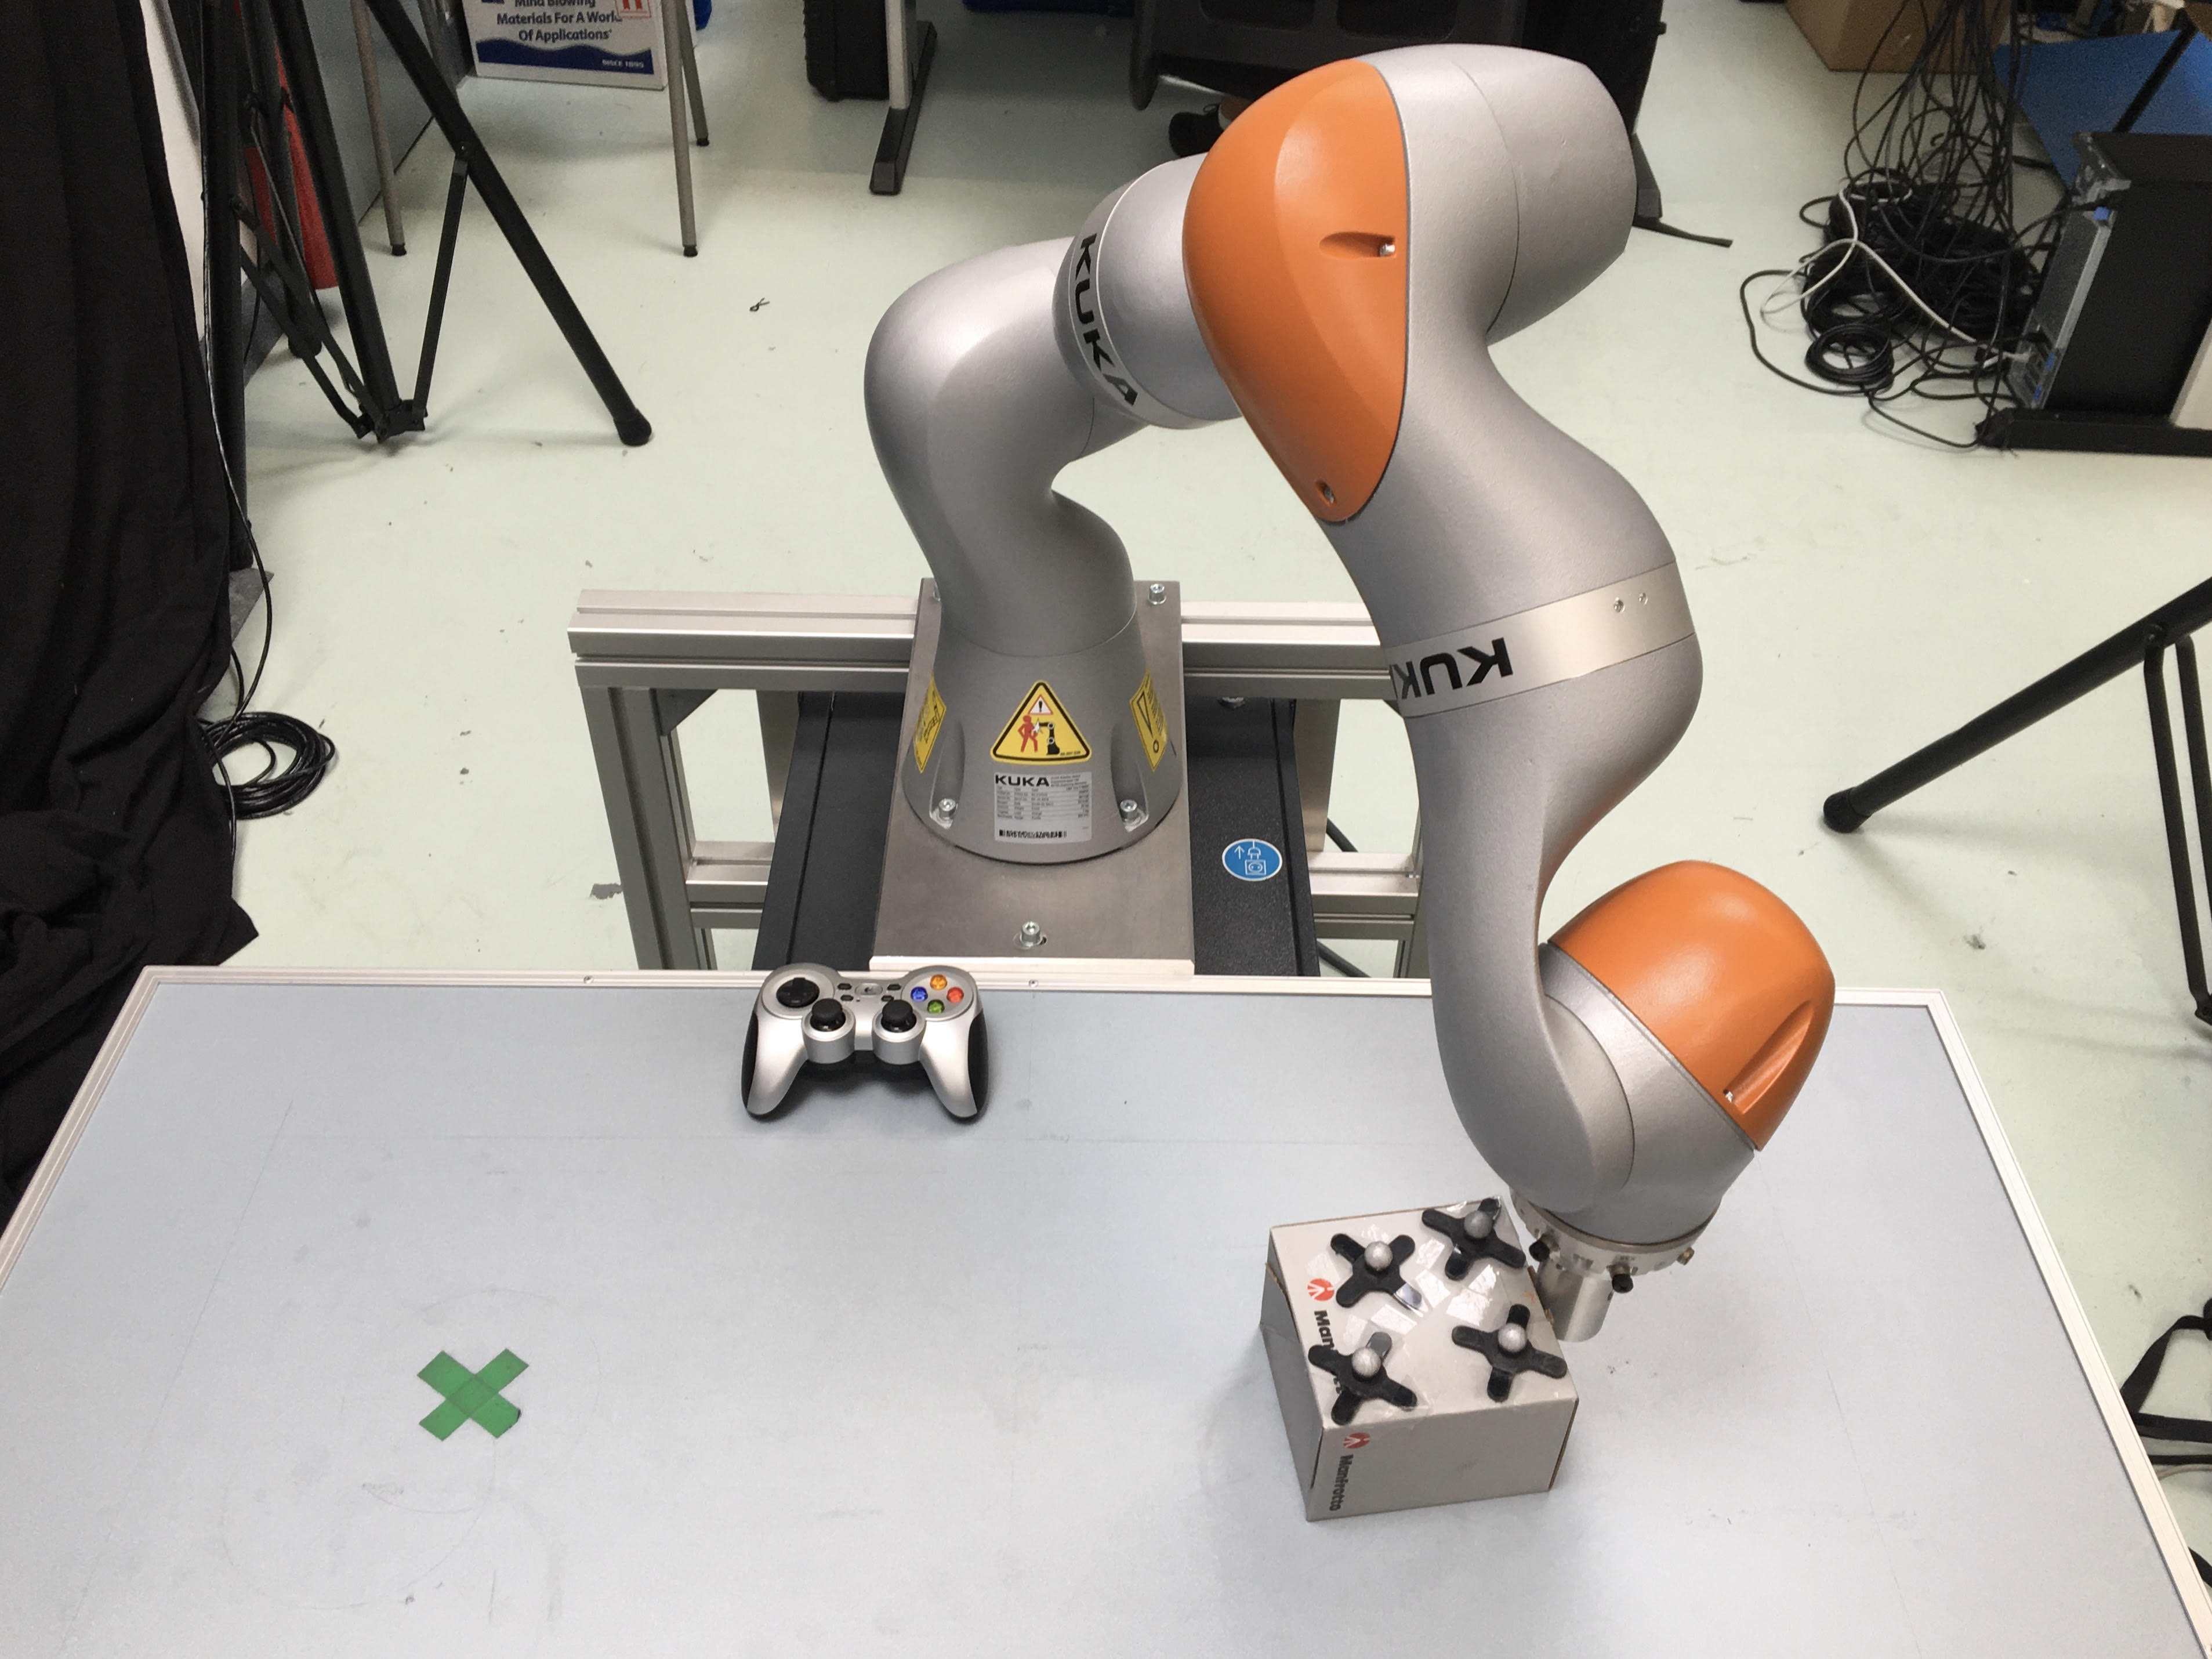
\includegraphics[width=.7\textwidth]{figures/kukapush.jpg}
    \caption{Reinforcement Learning}
    \label{fig:reinforcement_learning}
\end{figure}


\subsection{Park a box}
\label{subsection:Park a box}

\chapter{Results}
\label{chapter:Results}

This chapter provides the results of the performed experiments. The first section focuses on the results obtained on a simulated environment using two tasks from the Meta-World benchmark \cite{metaworld}. Here, the contribution of R-CIdL is measured by comparing its performance to that of D-COACH for different conditions of replay buffer size $K$, parameter $e$ and type of state (absolute or relative positions).
Finally, the results of two planar manipulation tasks are shown to validate R-CIdL on a real setup.



\section{Results of simulated tasks}
\label{section:results_metaworld}

To evaluate the contribution of R-CIdL with respect to the baseline method D-COACH, we did experiments with a simulated teacher on the Meta-World tasks plate-slide-v2 and drawer-open-v2  presented in sections \ref{subsection:metaworld-hockey-task} and
\ref{subsection:metaworld-open-drawer-task} respectively. 

Running some initial experiments it was observed that the type of state has an important influence on the performance of the agents. For both tasks the state consists on the coordinates in the Cartesian axes of the end effector, the coordinates of the object and the coordinates of the goal position. In the case of the plate-slide-v2 task, the object refers to the puck whereas for the drawer-open-v2 task, the object is the handle of the drawer.
If the positions of the state are absolute, the state is then equal to $[[xyz_\text{end effector}], [xyz_\text{object}], [xyz_\text{goal}]]$ 
On the other hand, if the positions are relative, then the state is equal to $[[xyz_\text{object} - xyz_\text{end effector}], [xyz_\text{goal} - xyz_\text{object}]]$. In this last case when the positions are relative to each other, not only the number of dimensions decreases but it is easier for the neural network to generalize the task.

The results for both tasks are divide in two parts. The first one shows how robust is the proposed method R-CIdL to variations of the parameters $e$ and replay buffer size $K$ in comparison to D-COACH when the state is formed by relative positions. Once the best combination of $e$ and $K$ is obtained for both methods, the experiments are repeated with those same conditions but this time the agent learns with states formed by absolute positions. The parameters used for the policy and the human model are shown in table \ref{tab:hyperparameters}. Trainings are 75000 time steps long which is approximately equivalent to 15 minutes of simulated time as the MuJoco time step duration is 0.0125 seconds.

In order to evaluate the robustness of R-CIdL, three values of $e$ and three values of $K$ are chosen. For $e$, we chose 0.01, 0.1 and 1 as these values are within the range tried during the real experiments. The three sizes for the replay buffer are 3000, 15000 and 30000; The reason behind these values is that the simulated teacher sends about 30000 corrections signals, therefore these sizes correspond to 10\%, 50\%  and 100\% of the maximum average accumulated corrections at the end of the trainings. The plots in the next subsections show the average success per episode of 20 trainings where each policy is evaluated 5 times.



\subsection{Performance of task plate-slide-v2}
\label{subsection:Performance of task plate_slide_v2}




Figure \ref{fig:results_plate_slide_buffer_e} shows the average success per episode for the task plate-slide-v2 for different values of $e$ and buffer size when the positions are relative. There are three main conclusions that can be extracted. First, R-CIdl is overall much more robust to changes in both $e$ and buffer size $K$ and it is able to reach 100\% success around minute 6. Regarding D-COACH, $e$ is the parameter that has more influence being its worst performance when $e=0.01$. And regarding the buffer size $K$, the biggest buffer is the most detrimental and the smallest results in the best performance at the end of the training.
This was expected as in D-COACH the buffer contains information gathered by all the previous old versions of the policy that may not be useful for updating the current version of the policy.


 \begin{figure}[htpb]
  \centering
  \subfloat{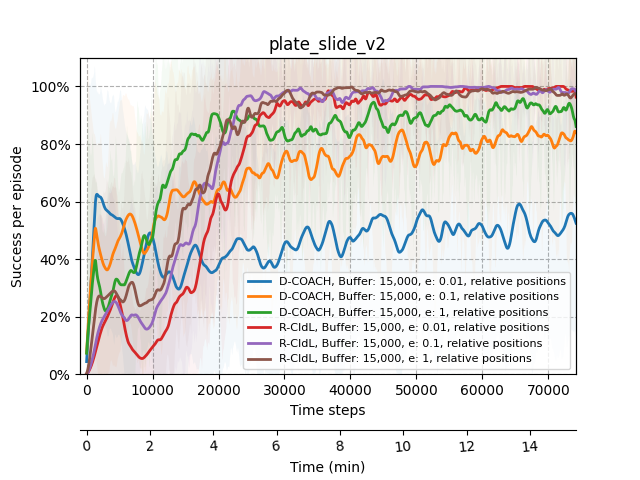
\includegraphics[width=0.5\textwidth]{figures/hockey_same_buffer_v2.png}\label{fig:plate_slide_same_buffer}}
   \hfill
  \subfloat{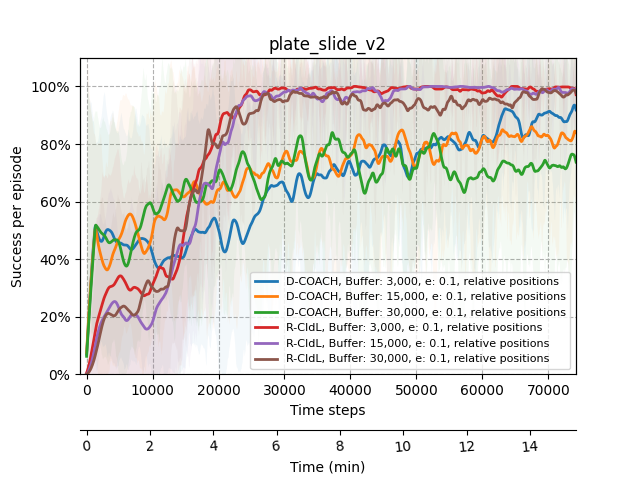
\includegraphics[width=0.5\textwidth]{figures/hockey_same_e_v2.png}\label{fig:plate_slide_same_e}}
  \caption{plate-slide-v2 results using a simulated teacher $P_h: \alpha = 0.9; \tau =  0.000015$. On the left, a comparison of the influence of the $e$ parameter on the baseline method D-COACH and on R-CIdL. On the right, a comparison of how different buffer sizes $K$ affect both methods.}
  \label{fig:results_plate_slide_buffer_e}
\end{figure}


      
From the previous analysis, the best combinations of buffer size $K$ and $e$ for both methods when positions are relative are $K=30000$ and $e=0.1$ for R-CIdL and $K=15000$ and $e=1$ for D-COACH. The experiments are repeated with the same values but this time considering absolute positions instead of relative ones. Figure \ref{fig:results_plate_slide_best} shows this comparison where R-CIdL, it is able to reach similar levels of performance as in the case of relative positions whereas the performance of D-COACH decreases a 20\%.



\begin{figure}[H]
    \centering
    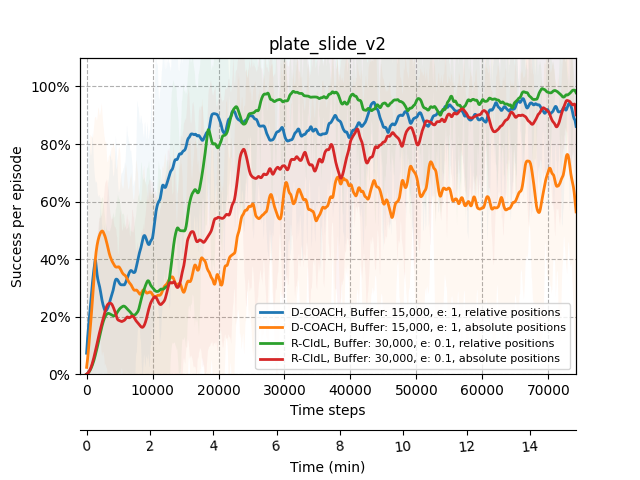
\includegraphics[width=.60\textwidth]{figures/hockey_best_v2.png}
    \caption{plate-slide-v2 results using a simulated teacher $P_h: \alpha = 0.9; \tau =  0.000015$. Comparison of the best performance of each method in relative positions, against their performances in absolute positions with the same conditions of $K$ and $e$.}
    \label{fig:results_plate_slide_best}
\end{figure}

\subsection{Performance of task drawer\_open\_v2}
\label{subsection:Performance of task drawer_open_v2}

Similar to previous task plate-slide-v2, figure \ref{fig:results_drawer_open_buffer_e} shows a comparison of the effect of different buffer sizes $K$ and different $e$. For the task drawer-open-v2, again, R-CIdL behaves more robust than D-COACH for the different conditions, being able to always reach performances close to 100 \%. On the other hand, D-COACH performs better in general than in the task plate-slide-v2 task but again, it can be observed that when the value of $e$ is small its performance decreases.


 \begin{figure}[H]
  \centering
  \subfloat{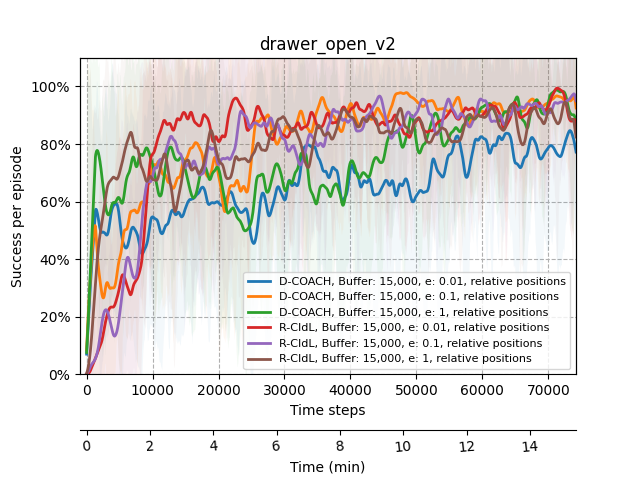
\includegraphics[width=0.5\textwidth]{figures/drawer_same_buffer_v2.png}\label{fig:drawer_open_same_e}}
   \hfill
  \subfloat{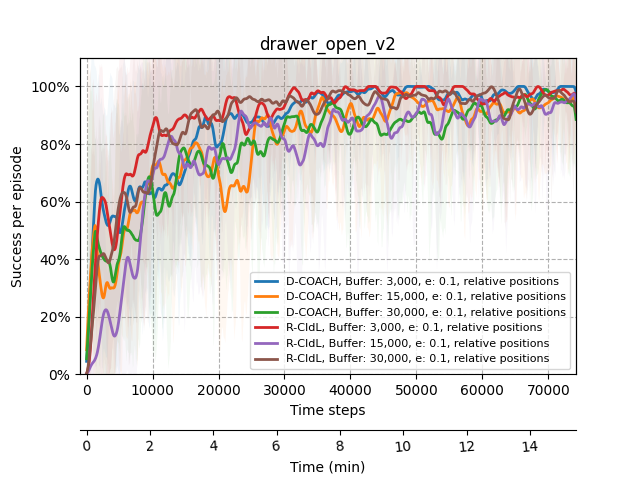
\includegraphics[width=0.5\textwidth]{figures/drawer_same_e_v2.png}\label{fig:drawer_open_same_buffer}}

  \caption{drawer-open-v2 results using a simulated teacher $P_h: \alpha = 0.9; \tau =  0.000015$. On the left, a comparison of the influence of the $e$ parameter on the baseline method D-COACH and on R-CIdL. On the right, a comparison of how different buffer sizes affect both methods.}
  \label{fig:results_drawer_open_buffer_e}
\end{figure}

From the previous analysis, the best combinations of buffer size $K$ and $e$ for both methods when positions are relative are $K=30000$ and $e=0.1$ for R-CIdL and $K=3000$ and $e=0.1$ for D-COACH. The experiments are repeated with the same values but this time considering absolute positions instead of relative ones. Figure \ref{fig:results_drawer_open_best}  shows this comparison where R-CIdL is able to reach similar levels of performance as in the case of relative positions. In the case of D-COACH, its performance soon reaches an average success of 70\% which increases just at the end of the training. Still, for D-COACH the difference in success between relative and absolute positions is remarkable.


\begin{figure}[H]
    \centering
    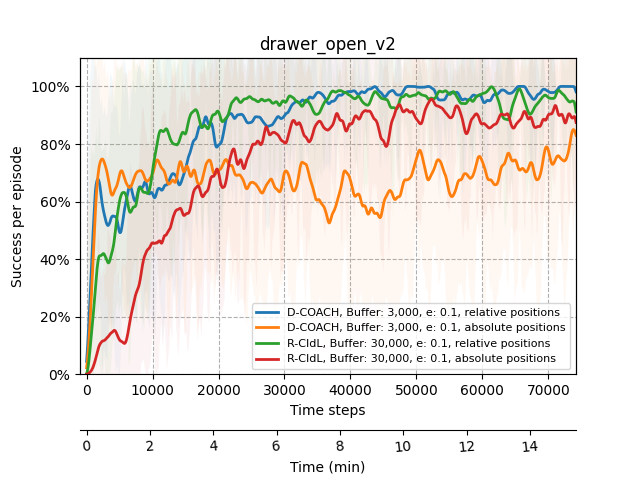
\includegraphics[width=.6\textwidth]{figures/drawer_best_v2.png}
    \caption{drawer\_open\_v2 results using a simulated teacher $P_h: \alpha = 0.9; \tau =  0.000015$. Comparison of the best performance of each method in relative positions, against their performances in absolute positions with the same conditions of buffer and $e$.}
    \label{fig:results_drawer_open_best}
\end{figure}


\section{Results of validation in real system}
\label{section:results_kuka}

To validate the proposed R-CIdL algorithm in a real system, we taught the 2 planar manipulation tasks described in sections \ref{subsection:Park a box} and \ref{subsection:Push box in a straight line}. The human teacher provided the necessary corrections to the position of the end effector with a joystick. In this subsection we show the results obtained for both tasks and because the objective is simply to validate R-CIdL, we did not performed comparisons with other methods. 


\subsection{Results for task "push a box"}
\label{subsection:results_kuka_push}
The result for the task "push a box" in figure \ref{fig:kukapush} shows the average success per episode of R-CIdL after a training of 60 minutes with a human teacher where 165 episodes were performed. Prior to the final training, some trials were done to adjust the value of $e$ which was found to work best with a value of 0.5. The replay buffer size $k$ for this task was set to 10000 which never got completely full because the human sends around 7300 correction signals.
The learning was evaluated every 5 episodes and every episode was on average 20 seconds long. At minute 23 approximately, the slope of the curve starts increasing until minute 35 when the success percentage reaches an average of 80\%.








% 165 episodes, evaluation every 5 episodes

% 7365 feedback signals
% Accumulated timesteps 13135
% e 0.5, buffer 10000 that never gets fully complete meaning that all the feedback provided is used to update the HumanModel
% Average timesteps per episode 72

% aprox 20 secs per episode

% at episode 60, 23 min the slope of the curve starts increasing until 130 episode (47 min) when the percentage of success is 80% aprox



\begin{figure}[H]
    \centering
    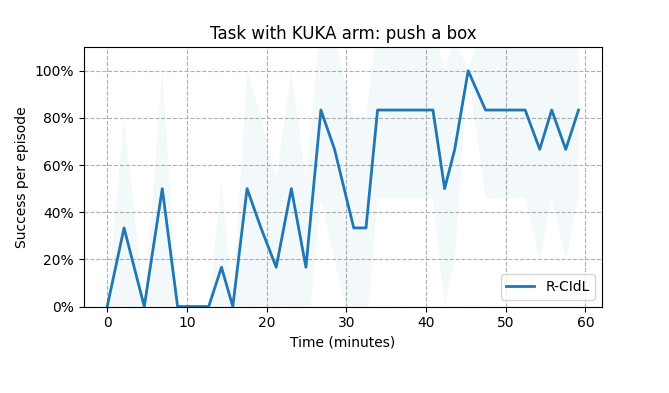
\includegraphics[width=.7\textwidth]{figures/push_1.png}
    \caption{Results of the task "push the box" with a human teacher.}
    \label{fig:kukapush}
\end{figure}

\subsection{Results for task "park a box"}
\label{subsection:results_kuka_park}

The results for the task "park a box" in figure \ref{fig:kukapark} show the average success per episode of R-CIdL after a training of 40 minutes with a human teacher where 65 episodes were performed. Prior to the final training, some trials were done to adjust the value of $e$ which was found to work best with a value of 0.3. The buffer size for this task was set to 10000 which never got completely full because the human sends around 3400 feedback signals.
The learning was evaluated every 5 episodes and every episode was on average 36 seconds long. Around minute 25 the performance increases drastically. This point in time corresponds with the moment that the R-CIdL agent learns to go around the corner (see third frame of figure \ref{fig:sequence-park-box}). Prior to that moment, all episodes logically fail. At episode 37, the performance reaches its maximum as all the following episodes are successful.



\begin{figure}[H]
    \centering
    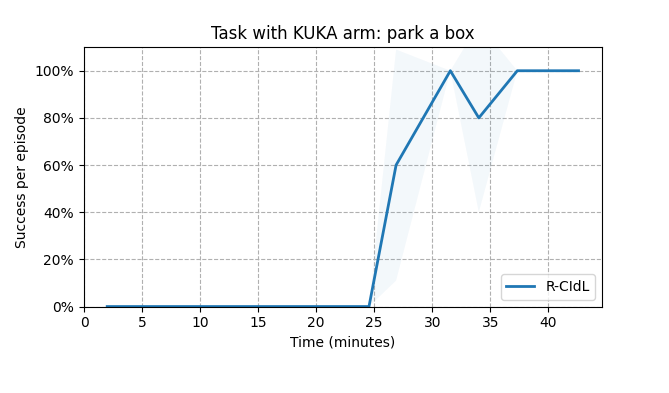
\includegraphics[width=.7\textwidth]{figures/park_1.png}
    \caption{Results of the task "park the box" with a human teacher.}
    \label{fig:kukapark}
\end{figure}

\chapter{Conclusion}
\label{chapter:conclusion}

\textbf{TODO}



BD-COACH successfully allows the usage of corrective feedback with neural networks in data intensive environments but it does not address the problem of data efficiency in the sense that it is not more data efficient than D-COACH. If the problem is too complex it can take a long time to train.

\begin{itemize}
  \item BD-COACH is computationally more expensive
  \item Advantage: With BD-COACH, some tasks require less feedback
  \item Advantage: With D-COACH it is necessary to adjust $e$ beforehand.
\end{itemize}
Interactive imitation learning refers to methods where a human teacher interacts with an agent during the learning process providing feedback to improve its behaviour. This type of learning may be preferable with respect to reinforcement learning techniques when dealing with real-world problems. This is especially true in the case of robotic applications where there are long training times and usu




%% Prevent urls running into margins in bibliography
\setcounter{biburlnumpenalty}{7000}
\setcounter{biburllcpenalty}{7000}
\setcounter{biburlucpenalty}{7000}

%% Bibliography is numeric style
\printbibliography[title=References]
\addcontentsline{toc}{chapter}{References}

%% Using letters for chapters
\appendix

\chapter{Appendix}
\label{appendix:Appendix}
\appendix




\section{Artificial Neural Networks}

An Artificial Neural Network or ANN is a computational model formed by a connection of artificial neurons arranged in structures called layers, \cite{ANN-graupe:2013}. Every ANN possesses three types of layers, the input layer, the hidden layer(s) and the output layer, see figure \ref{fig:ANN}.
\begin{figure}[H]
\centering
\begin{tikzpicture}[
plain/.style={
  draw=none,
  fill=none,
  },
net/.style={
  matrix of nodes,
  nodes={
    draw,
    circle,
    inner sep=10pt
    },
  nodes in empty cells,
  column sep=2cm,
  row sep=-9pt
  },
>=latex
]
\matrix[net] (mat)
{
|[plain]| \parbox{1.3cm}{\centering Input\\layer} & |[plain]| \parbox{1.3cm}{\centering Hidden\\layer} & |[plain]| \parbox{1.3cm}{\centering Output\\layer} \\
& |[plain]| \\
|[plain]| & \\
& |[plain]| \\
  |[plain]| & |[plain]| \\
& & \\
  |[plain]| & |[plain]| \\
& |[plain]| \\
  |[plain]| & \\
& |[plain]| \\    };
\foreach \ai [count=\mi ]in {2,4,...,10}
  \draw[<-] (mat-\ai-1) -- node[above] {Input \mi} +(-2cm,0);
\foreach \ai in {2,4,...,10}
{\foreach \aii in {3,6,9}
  \draw[->] (mat-\ai-1) -- (mat-\aii-2);
}
\foreach \ai in {3,6,9}
  \draw[->] (mat-\ai-2) -- (mat-6-3);
\draw[->] (mat-6-3) -- node[above] {Ouput} +(2cm,0);
\end{tikzpicture}
\caption{Diagram of an Artificial Neural Network, \cite{NN-tikz}} \label{fig:ANN}
\end{figure}





An artificial neuron, see figure \ref{fig:neuron}, is the simplest element of an ANN. Similar to a biological neuron, an artificial neuron has input connections through which it receives external stimuli, the input data $x$, \cite{ANN-graupe:2013}; With these inputs, the neuron makes a computation and generates an output value. This computation is a weighted sum of the input data where the weights $w$ are the parameters of the model that have to be adjusted in order for the model to learn. Furthermore, there is an additional input connection to the neuron, the parameter bias $b$ that also gets added to the weighted sum, $wx + b$. The final element of the artificial neuron is the activation function $f$ that takes as input the previous weighted sum and distorts it by adding non-linear deformations, $f(wx + b)$.

\begin{figure}[H]
\centering
\begin{tikzpicture}[
init/.style={
  draw,
  circle,
  inner sep=2pt,
  font=\Huge,
  join = by -latex
},
squa/.style={
  draw,
  inner sep=2pt,
  font=\Large,
  join = by -latex
},
start chain=2,node distance=13mm
]
\node[on chain=2] 
  (x2) {$x_2$};
\node[on chain=2,join=by o-latex] 
  {$w_2$};
\node[on chain=2,init] (sigma) 
  {$\displaystyle\Sigma$};
\node[on chain=2,squa,label=above:{\parbox{2cm}{\centering Activation \\ function}}]   
  {$f$};
\node[on chain=2,label=above:Output,join=by -latex] 
  {$y$};
\begin{scope}[start chain=1]
\node[on chain=1] at (0,1.5cm) 
  (x1) {$x_1$};
\node[on chain=1,join=by o-latex] 
  (w1) {$w_1$};
\end{scope}
\begin{scope}[start chain=3]
\node[on chain=3] at (0,-1.5cm) 
  (x3) {$x_3$};
\node[on chain=3,label=below:Weights,join=by o-latex] 
  (w3) {$w_3$};
\end{scope}
\node[label=above:\parbox{2cm}{\centering Bias \\ $b$}] at (sigma|-w1) (b) {};

\draw[-latex] (w1) -- (sigma);
\draw[-latex] (w3) -- (sigma);
\draw[o-latex] (b) -- (sigma);

\draw[decorate,decoration={brace,mirror}] (x1.north west) -- node[left=10pt] {Inputs} (x3.south west);
\end{tikzpicture}
\caption{Neuron diagram, \cite{NN-tikz}} \label{fig:neuron}
\end{figure}

ANNs can be classified according to multiple taxonomies, one of them refers to the direction in which the data is propagated through the layers, giving as a result two main groups: feedforward neural networks (FNN) and recurrent neural networks (RNN), \cite{Classification-Artificial-Neural-Networks:2017}.

\subsection{Feedforward Neural Networks (FNNs)}

A feedworward neural network (FNN) is a type of artificial neural network where information flows in only one direction from the input layer to the output layer without going through any loop.
  \vspace{1mm} \\


\subsection{Recurrent Neural Networks (RNNs)}

Opposite to feedforward neural networks, recurrent neural networks (RNNs) propagate data both forwards and backwards through the layers endowing the model with memory. RNNs are specially useful when dealing with sequential or time dependent where some information underlays hidden, e.g., temporal information.

\vspace{5mm} 
\textbf{1. Vanilla RNN}

Vanilla RNNs are the simplest version of recurrent networks (Figure \ref{fig:rnn} shows an unrolled Vanilla RNN cell). The hidden state $h$ is a parameter whose dimension is defined by the user and it is this parameter $h$ the one that forms the recurrent connection within the cell. The hidden state at time $t$, $h_t$ is computed by adding the input data at that time, $x_t$, plus the hidden state from the previous time step $h_{t-1}$, see equation \ref{eq:vanilla_rnn}. It is precisely the fact of adding information from previous states, which makes the model able to remember.

%\input{rnn_tikz}

\begin{figure}[H]
    \centering
    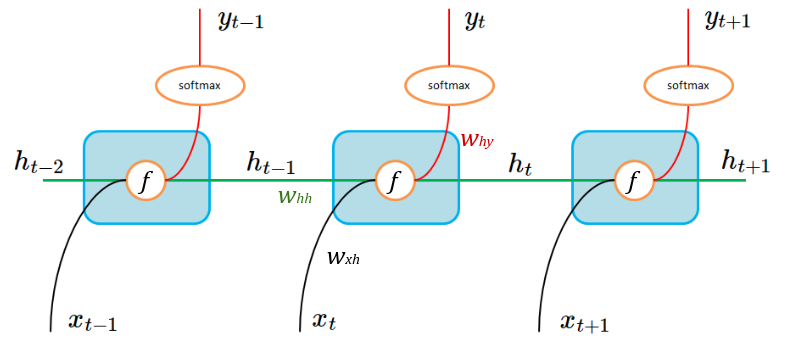
\includegraphics[width=.7\textwidth]{Figures/rnn.png}
    \caption{Vanilla Recurrent Neural Network, \cite{Vanilla-RNN-image}}
    \label{fig:rnn}
\end{figure}



\begin{equation}
h_t=tanh(W_{xh}x_t+W_{hh}h_{t−1})
\end{equation}


\begin{equation}
h_t = tanh\left(\begin{pmatrix}
W_{xh} & W_{hh}
\end{pmatrix}
\begin{pmatrix}
x_t \\
h_{t−1} \\
\end{pmatrix}\right)
\label{eq:vanilla_rnn}
\end{equation}


Vanilla RNNs suffer from a problem called vanishing/exploding gradient that makes them unable to work properly with big temporal horizons. Here is where long short-term memory (LSTM) come to play.

\vspace{5mm} 
\textbf{2. Long Short-Term Memory (LSTM)}

LSTMs are an improved version of the Vanilla RNN; They are able to learn long term dependencies by maintaining not only the hidden state $h$ but also a cell state $c$ which is the key of these networks. Furthermore, an LSTM cell includes four gates that control the flow of information to the cell state.

\subsection{Convolutional Neural Networks (CNNs)}


A convolutional neural network is a special type of ANN mostly used when the input data are images from which we want to extract information. To achieve this, filters (also called kernels) convolve on the input data producing feature maps. An example of how this convolution is done, can be seen in figure \ref{fig:cnn}. The filter (blue) slides over the input image (red) and at every location, a matrix multiplication takes place giving as a result a feature map (green). The objective of these CNNs is to learn the filters in order to detect patterns in the input images.
\begin{figure}[H]
\centering
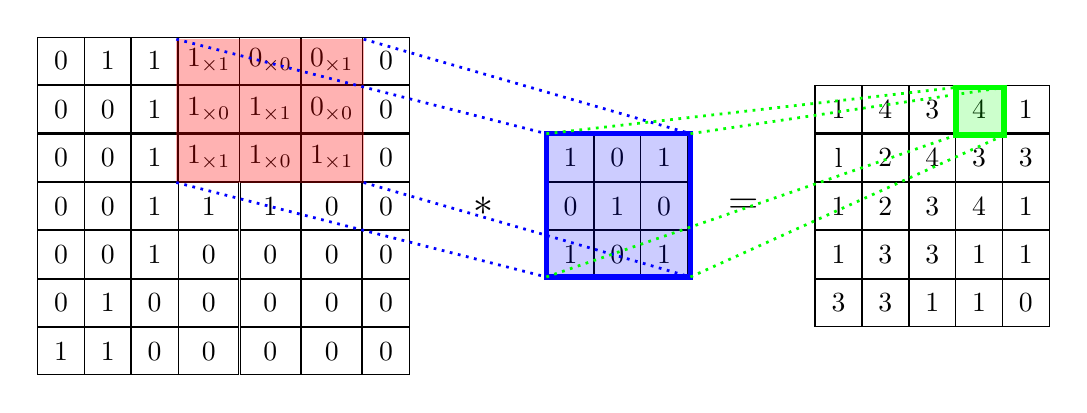
\begin{tikzpicture}[scale=1]

  \matrix [nodes=draw,column sep=-0.2mm, minimum size=6mm]
  {
    \node {0}; & \node{1}; & \node {1}; & \node{$1_{\times 1}$}; & \node{$0_{\times 0}$}; 
    & \node{$0_{\times 1}$}; & \node{0}; \\
    \node {0}; & \node{0}; & \node {1}; & \node{$1_{\times 0}$}; & \node{$1_{\times 1}$}; 
    & \node{$0_{\times 0}$}; & \node{0}; \\
    \node {0}; & \node{0}; & \node {1}; & \node{$1_{\times 1}$}; & \node{$1_{\times 0}$}; 
    & \node{$1_{\times 1}$}; & \node{0}; \\
    \node {0}; & \node{0}; & \node {1}; & \node{\, 1 \,}; & \node{\, 1 \, }; 
    & \node{\, 0 \,}; & \node{0}; \\
    \node {0}; & \node{0}; & \node {1}; & \node{\, 0 \, }; & \node{\, 0 \, }; 
    & \node{\, 0 \,}; & \node{0}; \\
    \node {0}; & \node{1}; & \node {0}; & \node{\, 0 \, }; & \node{\, 0 \, }; 
    & \node{\, 0 \,}; & \node{0}; \\
    \node {1}; & \node{1}; & \node {0}; & \node{\, 0 \,}; & \node{\, 0 \, }; 
    & \node{\, 0 \,}; & \node{0}; \\
  };


  % coordinates for coloring filter in array
  \coordinate (A) at (-0.6,0.3);
  \coordinate (B) at (1.78,0.3);
  \coordinate (C) at (1.78,2.12);
  \coordinate (D) at (-0.6,2.12);
  \fill[red, opacity=0.3] (A)--(B)--(C)--(D)--cycle;
  \begin{scope}[shift={(3.3,0)}]
    \node[] at (0,0) {\Large $\ast$};
  \end{scope}[shift={(2.5,0)}]

  \begin{scope}[shift={(5,0)}]

    %\matrix [matrix of math nodes,left delimiter={[},right
    %delimiter={]}]
    \matrix [nodes=draw,column sep=-0.2mm, minimum size=6mm]
    {
      \node{1};  & \node{0};   & \node{1};  \\
      \node{0};  & \node{1};   & \node{0};  \\
      \node{1}; & \node{0}; & \node{1}; \\
    };
    \coordinate (A1) at (-0.9,-0.9);
    \coordinate (B1) at (0.93,-0.9);
    \coordinate (C1) at (0.93,0.92);
    \coordinate (D1) at (-0.9,0.92);
    \fill[blue, opacity=0.2] (A1)--(B1)--(C1)--(D1)--cycle;
    \draw[blue, line width=2] (A1)--(B1)--(C1)--(D1)--cycle;
  \end{scope}

  \draw[dotted, line width=1, color=blue] (A)--(A1);
  \draw[dotted, line width=1, color=blue] (B)--(B1);
  \draw[dotted, line width=1, color=blue] (C)--(C1);
  \draw[dotted, line width=1, color=blue] (D)--(D1);

  \begin{scope}[shift={(6.6,0)}]
    \node[] at (0,0) {\Large $=$};
  \end{scope}[shift={(2.5,0)}]

  \begin{scope}[shift={(9,0)}]

    %\matrix [matrix of math nodes,left delimiter={[},right
    %delimiter={]}]
    \matrix [nodes=draw,column sep=-0.2mm, minimum size=6mm]
    {
      \node{1};  & \node{4};   & \node{3}; & \node{4}; & \node{1};  \\
      \node{l};  & \node{2};   & \node{4}; & \node{3}; & \node{3};  \\
      \node{1}; & \node{2}; & \node{3}; & \node{4} ; & \node{1};  \\
      \node{1}; & \node{3}; & \node{3}; & \node{1} ; & \node{1};  \\
      \node{3}; & \node{3}; & \node{1}; & \node{1} ; & \node{0};  \\
    };
    \coordinate (A2) at (0.3,0.9);
    \coordinate (B2) at (0.91,0.9);
    \coordinate (C2) at (0.91,1.507);
    \coordinate (D2) at (0.3,1.507);
    \fill[green, opacity=0.2] (A2)--(B2)--(C2)--(D2)--cycle;
    \draw[green, line width=2] (A2)--(B2)--(C2)--(D2)--cycle;
  \end{scope}

  \draw[dotted, line width=1, color=green] (A1)--(A2);
  \draw[dotted, line width=1, color=green] (B1)--(B2);
  \draw[dotted, line width=1, color=green] (C1)--(C2);
  \draw[dotted, line width=1, color=green] (D1)--(D2);
\end{tikzpicture}
\caption{Example of kernel in a CNN, \cite{Convolutional-tikz}} \label{fig:cnn}
\end{figure}








\subsection{Autoencoders}

An autoencoder, see figure \ref{fig:autoencoder} is neural network technique whose objective is to learn how to reduce the dimensionality of the input data, normally images, without losing their most important features. To do this, an autoencoder has three main parts: An encoder $e$, a latent space $L$ and a decoder $d$. The encoder $e(x)$, takes the input data and encodes it into a latent space $L$, a space of lower dimensionality. Then, the decoder takes this $L$ as input, and tries to reconstruct it so the output of the decoder is as similar as possible to the input $x$. The more similar is $\hat{x}$ to $x$, the better the relevant features have been captured into the latent space.

\begin{figure}[H]
\centering
\tikzset{arrow/.style={-stealth, thick, draw=gray!80!black}}

\begin{tikzpicture}
%     \draw[help lines](0,-5) grid (10,5);  
     
	\node[fill=blue!20, minimum width=0.5cm, minimum height=3.5cm] (X) at (0,0) {$\mathbf x$};
	
	\draw[fill=white!20] ([xshift=0.5cm]X.north east) -- ([xshift=2.5cm,yshift=0.5cm]X.east) -- ([xshift=2.5cm,yshift=-0.5cm]X.east) -- ([xshift=0.5cm]X.south east) -- cycle; 
	\node at (1.75,0) {\textsc{Encoder}};
	
	\node[fill=red!20, minimum width=0.5cm, minimum height=1.0cm] (Z) at (3.5cm,0) {$\mathbf L$};
	
	\draw[fill=white!20] ([xshift=0.5cm]Z.north east) -- ([xshift=2.5cm,yshift=1.25cm]Z.north east) -- ([xshift=2.5cm,yshift=-1.25cm]Z.south east) -- ([xshift=0.5cm]Z.south east) -- cycle;
	\node at (5.25,0) {\textsc{Decoder}};
	
	\node[fill=blue!20, minimum width=0.5cm, minimum height=3.5cm] (Xp) at (7,0) {$\mathbf{\hat{x}}$};
	
	\draw[arrow] (X.east) -- ([xshift=0.5cm]X.east);
	\draw[arrow] ([xshift=-0.5cm]Z.west) -- (Z.west);
	\draw[arrow] (Z.east) -- ([xshift=0.5cm]Z.east);
	\draw[arrow] ([xshift=-0.5cm]Xp.west) -- (Xp.west);
     
\end{tikzpicture}
\caption{Autoencoder, \cite{Autoencoder-tikz}} \label{fig:autoencoder}
\end{figure}


\chapter{List of Imitation Learning algorithms}
\label{appendix:List of Imitation Learning algorithms}
%\appendix



In this section, we gather and briefly describe some Imitation Learning algorithms with the objective of later classify them according to the proposed definitions from the previous subsection.




\subsubsection*{Behavioural Cloning}
Behavioural cloning (BC) \cite{Behavioural-Cloning-Pomerleau:1991}, one of the oldest Imitation Learning frameworks, consists on directly learning a policy, via supervised learning, given a data set of demonstrations provided by a teacher. The main problem with BC is known as \textit{distribution mismatch} and it happens because at the moment that the learner agent deviates from the expert trajectory, it cannot recover from that failure and go back to the expert trajectory. This provokes a cascade of errors that keep growing because the agent does not know how to act in those states that have not been visited by the expert \cite{Global-overview-Attia:2018}.

\subsubsection*{Inverse Reinforcement Learning methods}
Inverse Reinforcement Learning (IRL) is two-step approach for learning from humans. First, based on demonstrations provided by the human expert, the agent learns the reward function $R$ that best explains the behaviour of the human. Then, with this reward function, the optimal policy is learnt using RL methods \cite{inverse-reinforcement-learning}.

\subsubsection*{Learning from human preferences methods}
Learning from human preferences, \cite{learning-from-human-preferences:2017}, \cite{learning-from-human-preferences:2018},  are methods where iteratively, a human decides which of several executions of a policy is better according to the goal of the task. Then, a reward function that explains the decisions of the human is found and with it and applying RL, the agent learns how to perform the task. The user continues deciding between executions and so,  the policy gradually improves.


\subsubsection*{DART}
DART (Disturbances for Augmenting Robot Trajectories) \cite{DART-Laskey:2017} is an algorithm close to behavioural cloning \cite{Behavioural-Cloning-Pomerleau:1991}. According to its authors is an off-policy imitation learning algorithm because, after the first expert's demonstration, it does not require to query the expert anymore. This method works by injecting noise into the supervisor's policy while demonstrating the task, in order to force visiting a wider region of the state space and get the recovery demonstrations, therefore reducing the problem of distribution mismatch.

\subsubsection*{SQIL}
SQIL (Soft Q Imitation Learning) \cite{SQIL-Reddy-Dragan-Levine:2019} is a variant of behavioural cloning that incentives the agent to match human demonstrations over a long horizon. SQIL uses reinforcement learning but does not learn a reward function, instead, when the agent matches a demonstrated action in a demonstrated state, it receives a reward of "1" and "0" for every other behaviour.

\subsubsection*{ValueDICE}
ValueDICE (Distribution Correction Estimation) \cite{ValueDICE-Kostrikov:2019}, is an off-policy imitation learning \cite{Laskey:phdthesis} that minimize the KL-divergence between the expert distribution and the distribution induced by the agent when interacting with the environment in a off-policy manner.

%% DAGGERS!%%%%%%%%%%%%%%%%%%%

\subsubsection*{DAgger}
DAgger (Data Aggregation) \cite{DAgger-Ross:2011} is one of the most well-known imitation learning algorithms and it was explained in-depth in Section \ref{subsubsection:on and off-policy Imitation Learning}. Many variants of DAgger exist and some of them are going to be commented on next.



\subsubsection*{DAgger by coaching}
DAgger by coaching \cite{DAgger-by-coaching-He-DaumeIII-Eisner:2012},  is a version of DAgger \cite{DAgger-Ross:2011} where the human teacher executes actions that are within learner’s ability. This means that when the agent is at a state far from the desired state, the teacher will not try to correct directly that difference but instead it will try to redirect the agent gradually \cite{Global-overview-Attia:2018}.


\subsubsection*{AggreVaTe}
AggreVaTe (Aggregate Values to Imitate) \cite{AggreVaTe-Ross-Bagnell:2014}, is a version of DAgger \cite{DAgger-Ross:2011}, that learns to choose actions that minimize the cost-to-go of the expert, 
\cite{Global-overview-Attia:2018}. The cost-to-go $Q$ is the cost of executing an action in a state and continue executing a policy for the next steps. The first iteration is the same as in DAgger, then for the next iterations,  at a time t, the cost-to-go $Q$ of taking an action in a state is observed and added to the the initial dataset $D$ together with the action and the state.



\subsubsection*{AggreVaTeD}
AggreVaTeD \cite{AggreVaTeD-Sun:2017} is a differentiable version of the AggreVaTe algorithm introduced by \cite{AggreVaTe-Ross-Bagnell:2014} that does not perform any data aggregation. It includes two gradient update procedures: An online gradient descent and a natural gradient update similar to exponential gradient descent.

\subsubsection*{SafeDAgger}
SafeDAgger \cite{SafeDAgger-Zhang-Cho:2016}, is a version of DAgger \cite{DAgger-Ross:2011}, that aims to reduce the burden of constantly querying the human teacher by incorporating a safety policy. This safety policy predicts the discrepancy between the teacher and the learner and it is only on those states where the discrepancy is high, that the teacher is queried.


\subsubsection*{DropoutDAgger}
DropoutDAgger \cite{DropoutDAgger} is a method similar to SafeDAgger \cite{SafeDAgger-Zhang-Cho:2016}. It uses the dropout technique to train the neural network policy applying $N$ random dropout masks. For each random configuration of the network, an action is obtained for the same input observation. Only if its distribution over actions has enough probability mass around the action suggested by the expert, the mean action of the novice is taken, otherwise the action of the expert is chosen. When the distribution of actions has high entropy it means that that region of the state-space is unfamiliar and therefore, it is safer to chose the action of the expert.

\subsubsection*{EnsembleDAgger}
EnsembleDAgger \cite{EnsembleDAgger-Menda:2019}, is an extension of DAgger where the learning agent only acts when two measures are compliant with two preset thresholds: The first measure is the \textit{discrepancy}, which is the same as in SafeDagger \cite{SafeDAgger-Zhang-Cho:2016}; discrepancy represents the deviation between the agent and the expert. The second measure is the \textit{doubt} which is the variance that indicates the familiarity of the agent with its current state; the doubt constrains the learner to only act in familiar states. 

\subsubsection*{ThriftyDAgger}
ThriftyDAgger \cite{ThriftyDAgger} is a method similar to SafeDagger \cite{SafeDAgger-Zhang-Cho:2016} and EnsembleDAgger \cite{EnsembleDAgger-Menda:2019} in the sense that it switches the control between the agent and the human supervisor depending on the novelty and the risk of a particular state. ThriftyDAgger proposes a novel metric for measuring the riskiness of a state which captures the likelihood that the agent cannot succeed in converging to the goal state.

\subsubsection*{SHIV}
SHIV (Svm-based reduction in Human InterVention) \cite{SHIV-Laskey:2016},  is a method similar to DAgger \cite{DAgger-Ross:2011} that differs from this one in the fact that the human teacher is not queried to provide labels for all the visited states but only when it is risky. The risk is described as distance to a boundary defined by a one class support vector machine.

\subsubsection*{Hierarchical Guidance DAgger}
Hierarchical guidance \cite{Hierarchical-guidance-Le:2018} is a framework for hierarchical problems where low level sub-tasks can be identified by an expert. The authors present two settings: In the first one, hierarchical imitation learning,  the teacher provides high-level feedback and only provides low-level feedback when needed. The second setting is a hybrid imitation–reinforcement learning where the teacher provides only high-level feedback and the learner uses reinforcement learning at the low level.



\subsubsection*{BAgger}
BAgger (Bayesian  dataset  Aggregation) \cite{BAgger-Cronrath:2018}, is an extension of DAgger \cite{DAgger-Ross:2011} that aims to increase safety and reduce expert burden by querying the expert only when there is risk of not being able to imitate the expert. BAgger trains a Bayesian neural network or a Gaussian process to predict the expected error between teacher and learner.


















\subsubsection*{SAIL}
SAIL (Safety-Aware Imitation Learning) \cite{SAIL-Xiong:2019}, is an extension of DAgger that aims to reduce the number of queries to the expert. Only when the confidence level of the learning agent is lower than a threshold, is the expert queried. The expert continues providing labels until the confidence in all states is again higher than a threshold. Then, an uncertainty based approach decides whether or not continue querying the expert.

\subsubsection*{Retrospective DAgger}
Retrospective DAgger \cite{Retrospective-DAgger-song:2019}, is a version of the DAgger \cite{DAgger-Ross:2011} algorithm, designed for combinatorial search spaces. The policy learns from its mistakes by learning from retrospective inspections of its own roll-outs.  

\subsubsection*{HG-DAgger}
HG-DAgger (Human-Gated Data Aggregation) \cite{HG-DAgger-Kelly:2019}, is a version of DAgger \cite{DAgger-Ross:2011} that includes a gating function controlled by the expert; when the expert teacher detects that the agent is at a unsafe region of the state space, the expert takes control and leads the learning agent to a safe region of the state space.

\subsubsection*{EIL}
EIL (Expert Intervention Learning) \cite{EIL-Spencer:2020}, is an algorithm similar to HG-Dagger, that allows the teacher to take the control of the agent when needed. In HG-Dagger,  the labels that the human provides when taking control (explicit feedback) are used to update the data set. On the other hand, EIL not only uses this explicit feedback but also the implicit feedback which are those actions that the human does not correct because the agent is already behaving correctly. Finally, EIL also takes into account the timing, meaning when the feedback was provided.

\subsubsection*{FIRE}
FIRE (Failure Identification to Reduce Expert burden) \cite{FIRE-ablett:2020}, is an algorithm similar to HG-Dagger that incorporates the ability of notifying the expert when the agent is at a unsafe state. FIRE has a  failure predictor that classifies expert and non-expert data and predicts when a failure may occur. When this happens, the policy stops and if the human agrees with the prediction, he/she teleoperates the agent back to a safe state.

\subsubsection*{IWR}
IWR (Intervention Weighted Regression) \cite{IWR-mandlekar:2020} is an algorithm similar to FIRE, that focuses on \textit{bottlenecks} regions, that is, those states where it is necessary a sequence of precise actions. IWR keeps two different data sets, one with data provided by the human when intervening in a trajectory (mostly during bottleneck regions), and another one for the rest of the trajectory when the human does not intervene. During training, the two data sets are equally sampled which re-weights  the data distribution to reinforce those labels provided by the human  during bottleneck regions, while the data sampled from the non-intervention data set
keeps the policy close to previous policy iterations \cite{IWR-mandlekar:2020} .



\subsubsection*{DA-RB}
DA-RB (DAgger Replay Buffer) \cite{DA-RB-Prakash:2020}, is an extension of the DAgger algorithm \cite{DAgger-Ross:2011} that incorporate an additional replay buffer with the aim of controlling, in the data set, the proportion of data provided by the human and data gathered by the agent. This buffer is said to help the policy to focus on its weaker behaviours.




 
 \subsubsection*{COACH}
COACH (COrrective Advice Communicated by Humans) \cite{COACH-Celemin-Ruiz-del-Solar:2015}, is an algorithm designed for non-expert humans where feedback is provided as a binary signal interpreted as an increase or decrease of the value of an action.  The feedback is immediately used for updating the policy which makes it easy for the teacher to observe the change in the behaviour of the agent and continue providing further corrections. When a sequence of corrections has the same sign, it indicates that the correction to be made has a large magnitude. Opposite, if the signal alternates signs, the teacher is trying to make smaller corrections around a certain state. Furthermore, COACH includes a Human Feedback Model that helps to interpret and adapt the corrections.
This algorithm, and more specifically its deep version \cite{D-COACH-Dattari-Celemin-Ruiz-del-Solar-Kober:2018} are the main focus of this master thesis.

\subsubsection*{D-COACH}
D-COACH (Deep COrrective Advice Communicated by Humans) \cite{D-COACH-Dattari-Celemin-Ruiz-del-Solar-Kober:2018} is the deep learning version of the COACH algorithm \cite{COACH-Celemin-Ruiz-del-Solar:2015}. It uses artificial neural networks to represent the policy and includes a buffer to replay recent experiences. As already mentioned, this algorithm is the starting point of the present master thesis.



\subsubsection*{Advise}
Advise \cite{Advise-Griffith-et-al:2013}, is a policy shaping approach where the human teacher feedback is interpreted as direct policy labels; example of feedback could be \say{this is right} or \say{this is wrong} given an action taken by the agent. Advise also takes into account that the human feedback can be inconsistent and that correct feedback is provided with a probability $C$. Advise uses this probability and the Bayes rule to represent the human feedback policy \cite{leveraging-human-guidance:2019}.

\subsubsection*{I-SABL}
I-SABL (Inferring Strategy-Aware Bayesian Learning) \cite{I-SABL-Loftin:2016}, which is most similar to Advise \cite{Advise-Griffith-et-al:2013} uses expectation-maximization to calculate the best action. With this method, if the learning agent takes an optimal action, the human teacher provides positive feedback, otherwise, the human provides negative feedback \cite{leveraging-human-guidance:2019}.


\subsubsection*{ABLUF}
ABLUF (Adaptive Bayesian Learning with Uncertain Feedback) \cite{ABLUF-he:2020}, is based on expectation maximization algorithms, and it is similar to I-SABL \cite{I-SABL-Loftin:2016}. However, whereas I-SABL assumes that the expert only provides positive feedback when the agent takes an optimal action, ABLUF models the human feedback as a probability distribution, where the probability of providing positive or negative feedback, increases or decreases with respect to the distance between the action taken and the optimal action.



\subsubsection*{TAMER}
In the TAMER (Training an Agent Manually via Evaluative Reinforcement) framework \cite{TAMER-Knox-Stone:2009}, the teacher is seen as a reward function that maps the actions of the agent to negative, neutral or positive feedback. This kind of feedback is called evaluative feedback because the teacher evaluates how good or bad is the action taken by the agent. This reward function replaces the rewards provided by the environment in a classical reinforcement learning problem \cite{leveraging-human-guidance:2019}.
 

\subsubsection*{Deep TAMER}
Deep TAMER \cite{DeepTAMER-Warnell-et-al:2018} is a version of the TAMER framework \cite{TAMER-Knox-Stone:2009} where the policy is represented with a deep neural network.

\subsubsection*{DQN-TAMER}
DQN-TAMER \cite{DQN-TAMER-Arakawa:2018}, is a combination of the TAMER framework \cite{TAMER-Knox-Stone:2009} with Deep Q-Network (DQN). The original TAMER framework does not take into account the environment reward, but DQN-TAMER trains a DQN agent and a TAMER agent, and the final decision policy is a weighted average of the policies from both agents \cite{leveraging-human-guidance:2019}.

\subsubsection*{Convergent Actor-Critic by Humans}
Convergent Actor-Critic by Humans \cite{fakeCOACH-MacGlashan-Ho-Loftin:2017}, is an algorithm inspired in TAMER \cite{TAMER-Knox-Stone:2009} that differs from this one in that fact that TAMER interprets human feedback as a reward function independent of the agent’s current policy \cite{leveraging-human-guidance:2019}. 
Contrary, Convergent Actor-Critic by Humans assumes that human feedback depends on the agent's current policy and that it should be interpreted as the advantage function that tells how much better or worse when deviating from the agent’s current policy.

\subsubsection*{FRESH}
FRESH (Feedback-based REward SHaping) \cite{FRESH-xiao:2020}, is similar to Deep-TAMER \cite{DeepTAMER-Warnell-et-al:2018} but unlike Deep-TAMER, FRESH takes into account the reward from the environment.



\subsubsection*{LOKI}
LOKI (Locally Optimal search after K-step Imitation) \cite{LOKI-Cheng:2018}, is an algorithm that has two phases: A first imitation learning phase and a second reinforcement learning phase. First, it randomly picks a number within a range and performs that number of online imitation learning steps. Then, in the reinforcement learning phase, it improves the policy with a policy gradient RL method.










\subsubsection*{AOR}
AOR (Adaptive On-Policy Regularization) \cite{AOR-lee-laskey:2019}, is an algorithm that uses dynamic regret which measures performance of a policy at each iteration. Dynamic regret compares the current  policy  against  the  best  it  could  be  on  its  distribution with  respect  to  the  expert \cite{Dynamic-regret-Laskey:2018}.  

















\subsubsection*{Cycle-of-Learning}
Cycle-of-Learning \cite{Cycle-of-Learning-waytowich:2018},  is a framework that allows to switch between multiple types of human interventions when teaching an agent. Human interactions are divided in three categories arranged from more human control to less human control: Learning from human demonstration, learning from human intervention and learning from human evaluation. As the learning task progresses in time and the agent improves, less human intervention is required and therefore the algorithm switches to the following type of intervention technique.





\end{document}
